%%%%%%%%%%%%%%%%%%%%%%%%%%% asme2e.tex %%%%%%%%%%%%%%%%%%%%%%%%%%%%%%%
% Template for producing ASME-format articles using LaTeX            %
% Written by   Harry H. Cheng                                        %
%              Integration Engineering Laboratory                    %
%              Department of Mechanical and Aeronautical Engineering %
%              University of California                              %
%              Davis, CA 95616                                       %
%              Tel: (530) 752-5020 (office)                          %
%                   (530) 752-1028 (lab)                             %
%              Fax: (530) 752-4158                                   %
%              Email: hhcheng@ucdavis.edu                            %
%              WWW:   http://iel.ucdavis.edu/people/cheng.html       %
%              May 7, 1994                                           %
% Modified: February 16, 2001 by Harry H. Cheng                      %
% Modified: January  01, 2003 by Geoffrey R. Shiflett                %
% Use at your own risk, send complaints to /dev/null                 %
%%%%%%%%%%%%%%%%%%%%%%%%%%%%%%%%%%%%%%%%%%%%%%%%%%%%%%%%%%%%%%%%%%%%%%

%%% use twocolumn and 10pt options with the asme2e format
\documentclass[twocolumn,10pt]{asme2e}
\special{papersize=8.5in,11in}

%% The class has several options
%  onecolumn/twocolumn - format for one or two columns per page
%  10pt/11pt/12pt - use 10, 11, or 12 point font
%  oneside/twoside - format for oneside/twosided printing
%  final/draft - format for final/draft copy
%  cleanfoot - take out copyright info in footer leave page number
%  cleanhead - take out the conference banner on the title page
%  titlepage/notitlepage - put in titlepage or leave out titlepage
%  
%% The default is oneside, onecolumn, 10pt, final
\usepackage{amsmath,amssymb,amsfonts}
\newtheorem{theorem}{Theorem}
\newtheorem{lemma}{Lemma}
\newtheorem{coro}{Corollary}
\newtheorem{conj}{Conjecture}
\newtheorem{definition}{Definition}

%=====todonotes===== %
\usepackage{todonotes}
\usepackage{soul}
\definecolor{smoothgreen}{rgb}{0.7,1,0.7}
\sethlcolor{smoothgreen}

\newcommand{\todopara}[1]{\vspace{0px} %
\todo[inline, color=black!10]{\textbf{[Paragraph:]} {#1}} %
}
\newcommand{\todonote}[1]{\vspace{0px} %
\todo[inline, color=green!30]{\textbf{[Note:]} {#1}} %
}
\newcommand{\todoQ}[1]{\vspace{0px} %
\todo[inline, color=orange!50]{\textbf{[Note:]} {#1}} %
}
\newcommand{\todohere}[1]{\hl{(\textbf{TODO:} #1)}}

\newcommand{\hidetodos}{
\renewcommand{\todopara}[1]{}
\renewcommand{\todonote}[1]{}
\renewcommand{\todoQ}[1]{}
\renewcommand{\todohere}[1]{}}

%\hidetodos

\usepackage{graphicx}
\usepackage{caption}
\usepackage{subcaption}

% draw diagonal line in table
%\usepackage{slashbox}

\usepackage[hidelinks,pdftex,pdfauthor={Chang Liu, Shih-Yuan Liu, Elena L. Carano, J. Karl Hedrick},pdftitle={A framework for autonomous vehicles with goal inference and task allocation capabilities to support peer collaboration with human agents}]{hyperref}

%=====Better Spacing==== %
\usepackage{microtype}
%===Discourage hyphenation===
\hyphenpenalty=1000
%\tolerance = 1000


\usepackage{tabularx}
%\newcolumntype{Y}{>{\centering\arraybackslash}X}


\usepackage[capitalize]{cleveref}
%\crefname{equation}{Eqn.}{Eqn.}
\crefname{equation}{}{}
\Crefname{equation}{Equation}{Equations}



%%% Replace here with information related to your conference
\confshortname{DSCC2015}
\conffullname{the ASME 2015 Dynamic Systems and Control Conference}

%%%%% for date in a single month, use
%\confdate{24-28}
%\confmonth{September}
%%%%% for date across two months, use
\confdate{October 28--30}
\confyear{2015}
\confcity{Columbus, Ohio}
\confcountry{USA}

%%% Replace DETC2009/MESA-12345 with the number supplied to you 
%%% by ASME for your paper.
\papernum{DSCC2015-9814}

%%% You need to remove 'DRAFT: ' in the title for the final submitted version.
%\title{DRAFT: Autonomous target search in a dynamic environment using Model Predictive Control}
\title{Model Predictive Control-Based Probabilistic Search Method for Autonomous Ground Robot In A Dynamic Environment}

%%% first author
\author{Chang Liu\thanks{Address all correspondence to this author.}
    \affiliation{
    Vehicle Dynamics \& Control Lab\\
	Dept. of Mechanical Engineering\\
	University of California, Berkeley\\
	Berkeley, CA 94709\\
    Email: changliu@berkeley.edu
    }	
    \and
    \tensfb{Shengbo Eben Li}
    \affiliation{		
    	Dept. of Automotive Engineering\\
    	Tsinghua University\\
    	Beijing, 100084 China\\
    	Email: lisb04@gmail.com
    }
    \and 
    \tensfb{J. Karl Hedrick}
    \affiliation{
    	Vehicle Dynamics \& Control Lab\\
    	Dept. of Mechanical Engineering\\
    	University of California, Berkeley\\
    	Berkeley, California, 94709\\
    	Email: khedrick@berkeley.edu
    }
}

%%% second author
%%% remove the following entry for single author papers
%%% add more entries for additional authors
%\author{Shengbo Eben Li
%	\affiliation{		
%		Dept. of Automotive Engineering\\
%		Tsinghua University\\
%		Beijing, 100084 China\\
%		Email: lisb04@gmail.com
%	}
%	\and 
%	\tensfb{J. Karl Hedrick}
%	\affiliation{
%		Vehicle Dynamics \& Control Lab\\
%		Dept. of Mechanical Engineering\\
%		University of California, Berkeley\\
%		Berkeley, California, 94709\\
%		Email: khedrick@berkeley.edu
%	}
%}


\begin{document}

\maketitle

\begin{abstract}
Target search using autonomous robots is an important application for both civil and military scenarios.
In this paper, a model predictive control (MPC)-based probabilistic search method is presented for a ground robot to localize a stationary target in a dynamic environment.
%a path planning method for an autonomous robot equipped with a binary sensor to search for a stationary target is proposed.
The robot is equipped with a binary sensor for target detection, of which the uncertainties of binary observation are modeled as a Gaussian function. 
Under the model predictive control framework, the probability map of the target is updated via the recursive Bayesian estimation and the collision avoidance with obstacles is enforced using barrier functions.
By approximating the updated probability map using a Gaussian Mixture Model, an analytical form of the objective function in the prediction horizon is derived,
%for maximizing the probability of target detection, 
which is promising to reduce the computation complexity compared to numerical integration methods.
%In addition, collision avoidance with obstacles is also enforced using the barrier functions.
The effectiveness of the proposed method is demonstrated by performing simulations in dynamic scenarios with both static and moving obstacles.
\end{abstract}


\section*{INTRODUCTION} \label{sec:intro}
%Autonomous target search using robots, such as unmanned vehicles, have received much interest in the last decade due to their promising applications in civil and military missions.
%%, including mapping, search and tracking operations.
%Traditionally, works on the autonomous target search are focused on developing path planning methods for unmanned air vehicles (UAVs) to effectively localize targets without considering collision avoidance with obstacles in the environment.
%%This has gained success and been applied to both civil and military applications.
%%A few research focuses on the autonomous target search using unmanned ground vehicles or robots.
%%Such ignorance of obstacles makes sense as UAVs usually maintain a high latitude when searching and  
%%However, few work has been focused on path planning methods that take into account obstacles and pedestrians in the search environment that automous robots should avoid colliding with.
%Success has been achieved that UAVs can collaboratively localize targets using decentralized planning by exchanging each UAV's sensor detection result and search path.
%However, two issues exist for autonomous target search.
%First, the search path planning process usually involves numerical integration over large state space for solving an optimization problem, the objective function of which has no analytical formulation.
%Second, though the ignorance of collision avoidance with obstacles by UAVs is appropriate as UAVs usually maintain a high latitude in the air and no obstacle exist, this cannot apply to ground robots, since obstacles such as humans and constructions exist.
%%However, 
%%In many realistic situaitons, autonomous ground robots are necessary to be deployed for searching targets.
%%For example, in the search and rescue, autonomous ground robots can be used for searching survivors in indoor environments or areas where UAVs are not applicable, such as jungles.
%%In these scenarios, robots should take into account obstacles in the environment, such as humans and constructions, which implies the path planning methods for UAVs cannot apply directly to autonomous ground robots. 
%For example, autonomous ground robots searching objects in indoor environments should avoid collision with furnitures and humans. 
%%In these cases, those path planning methods may not apply.
%In this work, a path planning method that considers collision avoidance with obstacles in the environment is proposed for autonomous ground robots to perform the search operation.
%Besides, an analytical form of the objective function for computing the search path is derived. 
%This is promising to reduce the computation burden and can be applied for other autonomous target search problems.

%\todonote{think about reverting to the previous paragraph}
%In this work, we consider the problem of using an autonomous ground robot to search for a stationary target in a dynamic environment.
%This is an example of target search problems and its solution has many potential applications.
%For example, autonomous ground robots can be deployed in search and rescue missions for detecting survivors in disaster areas that are dangerous for human searchers.
%The robots should localize survivors in minimum time while avoiding collision with static or moving obstacles in the environment, such as buildings, vehicles and humans.
%A personal robot capable of searching can help people find and retrieve stuff indoors in daily life.

%Research on search problems can date back to 1940's, when the target search was treated as an area coverage problem,  \cite{koopman1946search}. 
%\todonote{consider including more references, such as from ICRA, IROS etc.}
Autonomous search using robots, such as unmanned vehicles, has attracted wide interest in the last decade.
This technique has been successfully employed for different applications, such as indoor search \cite{lau2006probabilistic}, marine search-and-rescue \cite{furukawa2006recursive} and object search-and-identify in the wilderness \cite{chung2009probabilistic}.
%Target search problems have been intensively investigated in the last decade due to the applications of unmanned vehicles for performing search and tracking operations.
Up until now, many algorithms have been developed for target search.
For example, Bourgault et al. \cite{bourgault2006optimal} proposed a Bayesian framework for searching and tracking a single target in an unconstrained environment.
%The belief of the target position is updated by using the recursive Bayesian estimation (RBE) to incorporate the UAV sensor observations.
%At each time, the search path follows the direction that maximizes the probability of detecting the target.
The one-step look-ahead scheme is used to either minimize mean-time-to-detection or maximize cumulative-probability-of-detection by following the descending gradient of objective function.
%The UAV search path is computed with the greedy method to maximize the probability of detecting the target at each time.
%Furukawa et al. \cite{furukawa2006recursive} extended the work in \cite{bourgault2006optimal} to multiple UAVs searching and tracking targets.
%Each UAV follows the path that maximizes the probability of detecting the target and the detection results are shared among UAVs.
%Tisdale et al. \cite{tisdale2009autonomous} utilized the recursive Bayesian estimation (RBE)-based search and tracking framework to perform the short-horizon path planning.
Tisdale et al. \cite{tisdale2009autonomous} utilized a receding horizon approach for a team of aerial vehicles to cooperatively search targets. 
A gradient routine is used to maximize the probability of detecting the target and a greedy method is used to sequentially decide vehicle motion for team collaboration.
Ryan et al. \cite{ryan2010particle} developed a control-based formulation to minimize the entropy of an estimated distribution for moving targets over a multiple-step horizon.
The prediction of conditional entropy is computed by sequential Monte Carlo method in the context of particle filtering.
Other examples can be found in \cite{kulich2014single,bonnie2012modelling,bertuccelli2006search}.
%To deal with the nonlinearity in the estimation process, a particle filter method is implemented in \cite{ryan2010particle}, which reduces the entropy of the uncertainty in the searched path.
%These research works all focus on using UAVs to search targets on the ground from the air.
%Therefore avoiding collision with obstacles in the environment is not considered.

In spite of aforementioned achievements, two issues still exist in the field of target search:
%Works on target search problems have provided powerful tool for robots to autonomously find and localize targets.
%However, two issues still exist for more efficient autonomous target search in a dynamic environment.
(1) many methods have either used one-step prediction to compute a myopic trajectory or solved a high-dimensional optimization problem. 
The former results in less effective search due to over-short planning horizon while the latter involves numerical integration over large state space;
%, which can result in high computation burden.
(2) few of them takes into account the issue of collision avoidance in dynamic environments that contain various types of moving obstacles.
%, which contains moving pedestrians, vehicles, etc.
%This makes sense as most of works on target search problems uses UAVs that searches from a high latitude in the air and no obstacle exist.
The negligence of collision avoidance is generally acceptable for aerial and marine search, but less suitable for ground environment, which may be crowded with pedestrians, motor vehicles, buildings and other inaccessible areas.
% such as using UAVs to search targets from a high altitude where no surrounding obstacle exists.
%However, such method cannot apply to the application considered in this paper that ground robots search in environments with obstacles such as buildings, vehicles and humans.
%However, such method cannot apply to cases
%such as the one considered in this paper, 
%where the environment contains obstacles that the robot searcher needs to avoid colliding with.
%Second, though the ignorance of collision avoidance with obstacles by UAVs is appropriate as UAVs usually maintain a high latitude in the air and no obstacle exist, this cannot apply to ground robots, since obstacles such as humans and constructions exist.

%Motion planning community usually focuses on designing a collision-free path in the environment containing static and dynamic obstacles.
%Optimization methods have been widely adopted to deal with such problems.
%Eele et al. \cite{eele2009path} applied the branch-and-bound optimization to find globally optimal path for vehicles with nonlinear dynamics to avoid fixed obstacles.
%Yokoyama et al. \cite{yokoyama2012path} applies the second-order cone programming relaxation to the originally non-convex motion planning problems for flights to avoid turbulent regions.
%The potential field method, since proposed by \cite{khatib1986real} in 1980s, has been widely applied for robot collision-free motion planning.
%The potential function is typically a sum of an attraction potential that drives the robot towards the goal configuration and a repulsion potential that pushes the robot away from obstacles.
%However, the design of the potential field needs much tunning for complex environments and the robot may get stuck in local minimum of the potential field.
%Therefore its applications are limited.
%In recent years, sampling-based motion planning methods, such as the Rapidly exploring random tree (RRT) \cite{lavalle2001randomized} and the Probabilistic roadmaps (PRMs) \cite{kavraki1996probabilistic}, have been used especially for problems with high dimensional state space.
%These methods typically constructs a motion tree from the starting state and expands it by adding collision-free feasible trajectories as new tree branches.
%However, since most works on motion planning focus on designing an optimal path between two states or a path that follows a given reference trajectory, they are not directly applicable to the search problem, in which no given destination or trajectory is provided beforehand.
%\cref{Binney} utilized the recursive greedy method, a graph-search based path planning algorithm, for a underwater glider to model the scalar field such 
%The glider should avoid high traffic areas 
%Kulich et al. \cite{kulich2014single} proposed a strategy for searching a stationary target in an environment with obstacles.
%It utilizes the grid-occupancy map to represent the target position and applied the frontier-based exploration method for planning paths.
%Though the grid-occupancy map can represent the exploration result by indicating whether a target exists within a grid, information about target positions cannot be as well utilized as using the probabilistic search formulation with RBE.

%\ and \ deals with the informative path planning, which are related to our problem.
%However, the underlying assumption about the Gaussian Process between different positions does not apply to our problem.

%In this work, we consider the problem of using an autonomous ground robot to search for a stationary target in a dynamic environment.
%This is an example of target search problems and its solution has many potential applications.
%For example, autonomous ground robots can be deployed in search and rescue missions for detecting survivors in disaster areas that are dangerous for human searchers.
%The robots should localize survivors in minimum time while avoiding collision with static or moving obstacles in the environment, such as buildings, vehicles and humans.

In this paper, we present a model predictive control-based probabilistic search method for an autonomous ground robot to localize a stationary target in the dynamic environment.
%Such method can have many potential applications.
%For example, autonomous ground robots can be deployed in search-and-rescue missions for detecting survivors in disaster areas that are dangerous for human searchers.
%The robots need to localize survivors while avoiding collision with static or moving obstacles, such as buildings, vehicles and humans, in the environment.
%, such as buildings, vehicles and humans.
%In the proposed method, the probabilistic search framework is utilized to construct a probability map to encode the information of the target position.
%A probability map is constructed to  and is updated using the particle filter method basd on the sensor detection results.
The main contributions of this paper include: 
(1) a receding horizon control problem is formulated by combining  the updated probability map of stationary target and barrier functions for safety concern, with the purpose of maximizing the probability of detecting the target while avoiding collision with surrounding obstacles;
%the MPC method is used to recursively compute a long-horizon optimal search path that maximizes the probability of detecting the target while guaranteeing no collision with obstacles in the dynamic environment.
%To enforce collision avoidance with obstacles, a barrier function, which was originally proposed for solving constrained optimization problems\cite{wright1999numerical}, is included in MPC.
(2) By approximating the updated probability map with a Gaussian Mixture Model, an analytical form of the objective function is derived for the search path optimization, which has the potential to allow a long prediction horizon and reduce the computation burden.
%Our contribution in this work is composed of two parts: first, we investigate an important application that autonomous ground robots search for targets while avoiding collision with obstacles in the environment;
%second, we derive a closed form objective function, which can also be utilized for search problem in other scenarios and is promising for reducing the computation complexity of the path planning.

The remainder of this paper is organized as follows: first, a receding-horizon control problem for target search is formulated;
% in \cref{sec:formulation}.
second, the method to update the probability map is described;
% in \cref{sec:update_prob_map}.
%In \cref{sec:explicit_form}, 
next, an analytical form of the objective function in MPC is derived and
% in \cref{sec:simulation}. 
lastly, simulation verification is presented.
% in \cref{sec:conclusion}.

\section*{PROBLEM FORMULATION}\label{sec:formulation}
Let $\mathit{S}=\left\lbrace x|x\in \mathbb{R}^2\right\rbrace $ denote a two-dimensional planar space containing one missing, but stationary target.
The exact target location is unknown but its probability map in $S$ is available.
An autonomous ground robot is tasked with localizing the target while needing to avoid colliding with surrounding obstacles.
The robot is assumed to be equipped with a binary sensor for detecting the stationary target and a perception system for detecting surrounding obstacles, such as buildings, pedestrians and vehicles. 
This assumption is reasonable because the target usually generates limited information to be accurately positioned. 
For example, in a rescue mission, a sound level sensor can only report whether there is a survivor within the detection range, while the motion of obstacles can be accurately measured and transmitted to the robot by using technologies such as Global Positioning System (GPS), geographic information system (GIS) or cellular network.


%Here we adopt the probabilisitc search framework, which will be descbribed in following sections.

\subsection*{Robot Motion Model}
%\todonote{it may be better to directly write the model using y}
A planar kinematic motion model is used for the robot, as shown in \cref{eqn:r_kinematics}:
\begin{subequations}\label{eqn:r_kinematics}
	\begin{align}
		y^R_{k+1}&=y^R_{k}+
		\begin{bmatrix}
		\cos{\theta^R_{k}} & 0\\
		\sin{\theta^R_{k}} & 0\\
		0 & 1
		\end{bmatrix}u^R_{k}\Delta t,\\
		y^R_k&=[x^R_k,\theta^R_k]\label{eqn:r_state},\\
		u^R_k&=[V^R_k,w^R_k]\label{eqn:r_input},
%		x^R_{k+1}&=x^R_k+V^R_k
%		\begin{bmatrix}
%			\cos{\theta^R_k}\\\
%			\sin{\theta^R_k}\
%		\end{bmatrix}\Delta t\\
%		\theta^R_{k+1}&=\theta^R_k+w^R_k\,\Delta t
	\end{align}
\end{subequations}
where $k$ is the time step; 
$y^R_{k}$ represents the state of the robot; 
$x^R_k$ and $\theta^R_k$ stand for the robot position and orientation in $\mathit{S}$, respectively;
$u^R_k$ is the control input;
$V^R_k$ denotes the robot velocity and $w^R_k$ represents the angular velocity;
$\Delta t$ is the sampling time.

%Define 
%\begin{subequations}
%	\begin{align}
%	
%	\end{align}
%\end{subequations} as the robot state at time $k$.
%The control input $u^R_k$ consist of the velocity $V^R_k$ and the angular velocity $w^R_k$ of the robot:
%\begin{equation}
%	u^R_k = [V^R_k,\theta^R_k]
%\end{equation}
Considering the actuator saturation, the control input is bounded by
\begin{equation*}
	u_m\le u^R_{k}\le u_M,
\end{equation*}
where $u_m$ and $u_M$ stand for the lower and upper bounds of the input, respectively.
\subsection*{Binary Sensor Model}
%A sensor model is used to update the probability map based on the robot sensor's observation result.
The binary sensor only gives two types of observation: $\mathbf{1}$ (the target is detected) and $\mathbf{0}$ (no target is detected).
%The former denotes that  by the sensor and the latter represents that .
%Different sensor models exist for binary sensors, depending on the types of the sensors.
Considering the sensor uncertainty, a Gaussian function is used to describe the probability that the target is detected:
%This model is similar to the one defined in.
\begin{equation}\label{eqn:sensor_model}
	P(z_k=\mathbf{1}|x^t,y_k^R;\Sigma^R) = \frac{c}{2\pi|\Sigma^R|^{\frac{1}{2}}}e^{-\frac{1}{2}(x^t-ay_k^R)^T{\Sigma^R}^{-1}(x^t-ay_k^R)},
\end{equation}
where $z_k$ is a random variable representing the sensor observation; 
$x^t$ denotes the target position; 
%$y_k^R$ stands for the state of the robot;
%\footnote{In this work, the robot sensor position and the robot position are assumed to be equivalent. This makes sense as the robot is modeled as a point-mass.}
%, as defined in \cref{eqn:r_state}; 
$\Sigma^R$ is a positive semidefinite covariance matrix; 
$a=[1,1,0]$ and thus $ay_k^R=x_k^R$, which is the robot position;
$c$ represents a scaling constant and is chosen as $c=2\pi|\Sigma^R|^{\frac{1}{2}}$ for normalization.
%This selection makes the probability of detection equal one when $x^t=x_k^R$, which means the robot can always detect the target when it is at the same position as the target.
\cref{fig:sensor_model1} shows the probability of "target is detected" in the 1-D case.
%The x-axis represents the target position and the sensor is placed at the origin.
%It should be noted that the sensor model need not to be a probability density function.
%Instead, it works as a likelihood function with the value between $0$ and $1$.
For the purpose of simplicity, the binary sensor is assumed to be homogeneous in all directions so that $\Sigma^R$ is a diagonal positive semidefinite matrix with two identical eigenvalues.
% and therefore the probability of detection does not depend on $\theta^R_k$, but on $x^R_k$ only.
A heterogeneous sensor can easily be accommodated by modifying $\Sigma^R$.

Correspondingly, the probability of "no target is detected" is
\begin{equation}\label{eqn:sensor_model_nD}
	P(z_k=\mathbf{0}|x^t,y_k^R;\Sigma^R) = 1-P(z_k=\mathbf{1}|x^t,y_k^R;\Sigma^R).
\end{equation}

The 1-D case is illustrated in \cref{fig:sensor_model2}.
Even though the sensor uncertainty \cref{eqn:sensor_model} is modeled as a Gaussian function, the binary observation is actually not a Gaussian process.
This fact is important for selecting the updating strategy of target probability map, which will be stated later.
\begin{figure}
	\begin{subfigure}[b]{0.2\textwidth}
		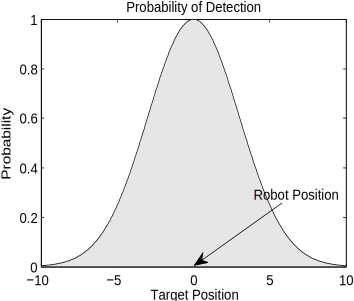
\includegraphics[width=\textwidth]{figures/PoD}
		\caption{}\label{fig:sensor_model1}
	\end{subfigure}
	\begin{subfigure}[b]{0.2\textwidth}
		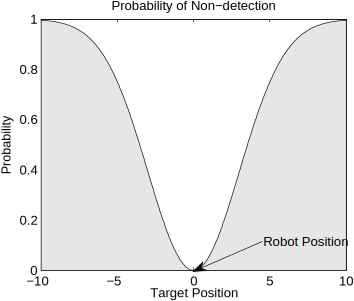
\includegraphics[width=\textwidth]{figures/PoND}
		\caption{}\label{fig:sensor_model2}
	\end{subfigure}
	\caption{\cref{fig:sensor_model1}: Probability of detection. \cref{fig:sensor_model2}: Probability of non-detection}
\end{figure}

\subsection*{Probability Map of The Stationary Target}
The exact target location is unknown but its probability map in $S$ is available.
The probability map is defined as $f_k(x^t)$, satisfying
%such that the probability that the target exists in an area $\Delta\in\mathit{S}$ equals
%\begin{equation}
%P(x\in \Delta) = \int_{\Delta} f(x)\,\mathrm{d}x
%\end{equation}
%and
%Let  be the probability map at time $k$.
\begin{equation*}
\int_{\mathit{S}} f_k(x^t)\,\mathrm{d}x^t = 1.
\end{equation*}

The probability map provides a tool to encode the belief about the target position.
As the robot continues searching, the probability map will be updated based on the binary observation.
%T=in \cref{sec:update_prob_map}.
Intuitively, an update strategy should fulfill the following functionalities: (1) the areas that have been searched but no target is found will reduce probability density;
(2) once the target is observed, the probability density in the searching area will increase.
The target is considered to be localized when the $l_2$-norm of covariance matrix of $f_k(x^t)$ is smaller than a given threshold.

%$f_k(x^t)$ is used in the objective function in MPC to compute a finite-horizon optimal path for the robot to search the target.

\subsection*{Probabilistic Search Using Model Predictive Control}
The receding-horizon control problem for target search is formulated under the model predictive control (MPC) framework, shown in \cref{eqn:mpc}. 
The main goal of this problem is to maximize the probability of detecting the target in the prediction horizon while avoiding collision with surrounding obstacles.
\begin{subequations}\label{eqn:mpc}
	\begin{align}
	\min_{u^R_{k:k+H-1}}\; & J(y^R_k,u^R_{k:k+H-1})=w_1J_{\text{pnd}}(y^R_k,u^R_{k:k+H-1})\notag\\&\qquad\qquad\qquad+w_2J_{\text{col}}(y^R_k,u^R_{k:k+H-1})\notag\\&\qquad\qquad\qquad+w_3J_{\text{trm}}(y^R_k,u^R_{k:k+H-1})\label{eqn:mpc_obj}\\
%	s.t. &\, y^R_{k+i+1}=g(y^R_{k+i},u^R_{k+i})\\
	s.t. &\quad
	y^R_{k+i+1}=y^R_{k+i}+
	\begin{bmatrix}
	\cos{\theta^R_{k+i}} & 0\\
	\sin{\theta^R_{k+i}} & 0\\
	0 & 1
	\end{bmatrix}u^R_{k+i}\Delta t,\\
%	&\,\theta^R_{k+1}=\theta^R_k+w^R_k\,\Delta t\\
	&\quad u_m\le u^R_{k+i}\le u_M,\\
%	&\,u^R_{k+i}\in \mathcal{U}\\
%	&\, y^R_{k+i+1}\in \mathcal{X}\\
	& \quad i=0,\dots,H-1,\notag
	\end{align}
\end{subequations}
where $H$ is the prediction horizon;
%$g(y^R_{k+i},u^R_{k+i})$ represents the robot motion model \cref{eqn:r_kinematics};
$u^R_{k:k+H-1}=[u^R_{k},\dots,u^R_{k+H-1}]$ is the set of control inputs in the prediction horizon.
%$\mathcal{X}$ and $\mathcal{U}$ are feasible sets for states and inputs.
At each step $k$, optimal control inputs $u^{R*}_{k:k+H-1}$ is calculated and the first input $u^{R*}_{k}$ is applied for robot control.
%MPC is suitable for the probabilistic search framework as it incorporates the updated probability map at each time step.
%The MPC, also called the Receding Horizon Control, is an iterative, finite horizon optimization approach.
%Each time an optimal control inputs for a finite horizon is obtained and only the first input is applied to the controlled system.
%Then the optimal control inputs are calculated at the updated system state after applyign the previous optimal input.

%Several types of objective functions for the target search problem have been proposed in literature, including the mutual information \cite{hoffmann2010mobile} and the expected time of detection \cite{furukawa2006recursive}.
The objective function is a weighted sum of three sub-functions: $J_{pnd},\,J_{col}\text{ and }J_{trm}$, namely, non-detection function, collision avoidance function and terminal cost function, respectively.
The first sub-function plays a major role in target detection while 
the second one enforces the robot to avoid collision with obstacles.
The third sub-function is used to guide the robot towards high probability density region, where the target is more likely to be located.
Note that the calculation of the first and third sub-functions depends on the target probability map, which is updated at each control step of MPC.
%which is updated by the recursive Bayesian estimation.
%which will be stated in the following section.

(1) The non-detection function is defined as
%It maximizes the probability of detecting the target for at least once in the finite horizon.
\begin{equation}\label{eqn:obj1}
J_\text{pnd}(y^R_k,u^R_{k:k+H-1})=P(z_{k+1:k+H}=\mathbf{0}|y^R_k,y^R_{k:k+H-1}),
\end{equation}
which actually represents the probability of "no-target-is-detected" in the prediction horizon.
%By minimizing \cref{eqn:obj1}, the robot maximizes the probability of detecting the target in the prediction horizon.
Traditionally, the calculation of \cref{eqn:obj1} incurs high computation burden because no analytical form exists and numerical integration over large state space is required.
This paper derives an analytical form for this sub-function by approximating the updated probability map as a Gaussian Mixture Model, which has the potential to allow the use of longer prediction horizon and reduce the computation burden.
%It is calculated based on the sensor model \cref{eqn:sensor_model} and the probablity map $f_k(x^t)$.
%Utilizing the deterministic robot model \cref{eqn:r_kinematics}, the robot state $[y^R_{k+1},\dots,y^R_{k+H}]$ can be obtained by applying $[u^R_{k},\dots,u^R_{k+H-1}]$ to $y^R_k$.
%For the purpose of simplicity, we use the notation $P(z_{k+1:k+H}=\mathbf{0}|y^R_k,y^R_{k+1:k+H})$ to replace $P(z_{k+1:k+H}=\mathbf{0}|y^R_{k},u^R_{k+1:k+H})$ in 
%Usually, an analytical form of \cref{eqn:obj1} does not exist.
%By approximating $f_k(x^t)$ with the Gaussian Mixture Model, we have obtained an analytical form for it, which will be described later.
%in \cref{sec:explicit_form}.
%Constraints in MPC include the robot kinematics model and collision avoidance requirements.

%As the robot searches in an environment containing obstacles, collision avoidance should be considered when planning the search path.
%\todonote{why non-cvx leads to high burden. why barrier function is good?}
(2) 
%Traditionally, collision avoidance requirements are formulated as non-convex constraints in an optimization problem\cite{yokoyama2012path,eele2009path}, which results in high computational complexity.
Collision avoidance is enforced by using barrier functions as
\begin{equation}\label{eqn:obj2}
J_\text{col}(y^R_k,u^R_{k:k+H-1}) = -\sum\limits_{i=1}^{H}(\sum\limits_{l=1}^{n_p}log(d^{Rp_l}_{k+i}-r^{Rp})+\sum\limits_{m=1}^{n_b}log(d^{Rb_m}_{k+i}-r^{Rb})),
\end{equation}
where $n_p$ and $n_b$ denote the number of moving and static obstacles, respectively;
$r^{Rp}$ and $r^{Rb}$ represent the safe distances;
$d^{Rp_l}_{k+i}\,(l=1,\dots,n_p)$ and $d^{Rb_m}_{k+i}\,(m=1,\dots,n_b)$ stand for Euclidean distances between obstacles and robot, defined as
\begin{subequations}%\label{eqn:dis_rho}
	\begin{align}
	d^{Rp_l}_{k+i}&=||x^R_{k+i}-\hat{x}^{p_l}_{k+j}||_2,\\
	d^{Rb_m}_{k+i}&=||x^R_{k+i}-x^{b_m}||_2,
	\end{align}
\end{subequations}
where $x^{b_m}$ represents the position of the $m^\text{th}$ static obstacle and $\hat{x}^{p_l}_{k+i}$ denotes the predicted position of the $l^\text{th}$ moving obstacle at time $k+i$.
%Traditionally, the barrier function approach is used in solving constrained optimization problem\cite{wright1999numerical}.
%\todonote{need to tell the benefit of the barrier function method. the barrier function method for collision avoidance have been used in other works\cite{panagou2013multi}.}
When the distance between the robot and an obstacle drops below the safe distance, \cref{eqn:obj2} will increase to infinity, which prohibits the robot from colliding with any obstacle.
%Prediction of moving obstacles' motion trajectory is necessary for the robot to avoid colliding with them.
Here a constant-velocity motion model is used to predict the future trajectory of moving obstacles, such as pedestrians and motor vehicles: 
%The moving obstacle motion prediction can be summarized as follows:
\begin{subequations}
	\begin{align}
	\hat{v}^{p_l}_k&=\frac{x^{p_l}_k-x^{p_l}_{k-1}}{\Delta t},\,l=1,\dots,n_p,\\
	\hat{x}^{p_l}_{k+i}&=x^{p_l}_k+i\hat{v}^{p_l}_k\Delta t,\,i=1,\dots,H,
	\end{align}
\end{subequations}
where $\hat{v}^{p_l}_k$ is the estimated velocity and $\hat{x}^{p_l}_{k+i}$ is the predicted position at time $k+i$.
%\todonote{need to change}
For more complex prediction methods, readers can refer to \cite{ferrer2014behavior,bruce2004better}.

(3) The terminal cost function $J_\text{trm} (y^R_{k},u^R_{k:k+H-1})$ is defined as
\begin{equation}\label{eqn:obj3}
J_\text{trm} (y^R_k,u^R_{k:k+H-1})=||x_{k+H}^R-x^M_k||_2,
\end{equation}
in which $x^M_K$ is the peak of the target probability map:
\begin{equation}
x^M_k = \arg\max_{x^t} f_k(x^t).
\end{equation}

%$f_k(x^t)$ represents the updated probability map at time $k$.
%stands for a segmentation of the environment $\mathit{S}$, obtained by the k-means clustering method\cite{keylist}.
The terminal cost function penalizes the distance between the robot and the probability peak.
Moreover, the weight $w_3$ can be adjusted based on the value of $J_\text{pnd} (y^R_{k-1},u^R_{k-1:k+H-2})$, i.e., $w_3=0$ when $J_\text{pnd} (y^R_{k-1},u^R_{k-1:k+H-2})>\epsilon$, where $\epsilon$ is a given threshold; otherwise, $w_3\neq 0$.
%which indicates that the robot is still in an area with low probability density.
This design is able to drive the robot out of local low probability density areas towards the position with high probability density.

%When the maximal probability density in the current area is less than $\epsilon$, the \cref{key} is added to the objective function and the robot tends to move to another area containing high probability.
%The second terminal function, shown in \cref{key}, guides the robot towards the high probability desnity region within current area.

%We have obtained the analytical forms of $J_\text{col}$ and $J_\text{trm}$.
%Usually, an analytical form of \cref{subsec:obj} does not exist.
%Utilizing We have obtained an analytical form for it, which will be described in .

%\section*{Methods}\label{sec:methods}
%In this section, the methods for the probabilistic search is described in detail.
%The particle filter method is applied for updating the probability map based on sensor detection results.
%A Gaussian Mixture Model (GMM) is calculated to approximate the probability map.
%Using the GMM, an analytical form of the ojective function is derived.


\section*{UPDATING THE PROBABILITY MAP}\label{sec:update_prob_map}
The recursive Bayesian framework is used to fuse binary sensor observations for updating the probability map of target position.
Since the observation of binary sensor is a non-Gaussian process, many filtering schemes, such as the Kalman filter\cite{kalman1960new,harvey1990forecasting} are precluded.
Thus, a particle filter-based scheme is utilized to implement the Bayesian framework.
%For numerical implementation, the particle filter is applied to calculate RBE considering the probabilistic sensor model.
%The updated probability map is then approximated as a Gaussian Mixture Model (GMM).

\subsection*{Recursive Bayesian Estimation (RBE)}
%Several well-known methods, such as , have been applied for target localization \cite{grocholsky2006cooperative}.
%These methods require measured target location as the input and therefore they are suitable for the situation that the target is always detected, but not for the binary observation.
%search problems as the target position is unknown and thus the target is unlikely to be detected at the early stage of the search process.
The Bayesian estimation provides a unified approach for estimating target position by applying the binary sensor data to a prior probability distribution. 
%that incorporates both the 'detection' and 'non-detection' results of binary sensor, which will be used in this paper to update the probability map.
%The target in this work is stationary.
%Therefore only the update step is necessary and no prediction step is needed.
%To illustrate the key steps in the updating procedure, we use $f_k(x)$ to represent the probability map at time $k$.
%Consider $f_k(x)$, the probability map at time $k$.
The probability map at time $k$ actually represents a conditional likelihood function of the target position.
% given the sensor observations up to:
\begin{equation}\label{eqn:prob_map}
f_k(x^t)=P(x^t|z_{1:k},y^R_{1:k}).
\end{equation}

%where $y^R_{1:k}$ are the robot states at time $1,\dots,k$ and $z_{1:k}$ are the corresponding observation results.
%The following formula updates $P(x^t|z_{1:k},y^R_{1:k})$ based on the observation $z_{k+1}$:
The sensor observation $z_{k+1}$ is applied to update $P(x^t|z_{1:k},y^R_{1:k})$:
\begin{equation}\label{eqn:update}
P(x^t|z_{1:k+1},y^R_{1:k+1})=\frac{P(z_{k+1}|x^t,y^R_{k+1})P(x^t|z_{1:k},y^R_{1:k})}{P(z_{k+1}|z_{1:k},y^R_{1:k+1})}.
\end{equation}

Actually, \cref{eqn:update} has been simplified by using the following two equalities:
\begin{subequations}
	\begin{align}
	P(z_{k+1}|x^t,z_{1:k},y^R_{1:k+1}) &= P(z_{k+1}|x^t,y^R_{k+1}),\label{eqn:cond_ind1}\\
	P(x^t|z_{1:k},y^R_{1:k+1})&=P(x^t|z_{1:k},y^R_{1:k}).\label{eqn:cond_ind2}
	\end{align}
\end{subequations}

This simplification is reasonable because of two conditional independences: (1) the sensor observation $z_{k+1}$ only depends on the target position $x^t$ and the robot state $y^R_{k+1}$;
(2) the estimation of target position $x^t$ is only affected by $z_{1:k}$ and $y^R_{1:k}$.
%Considering these, \cref{eqn:update} can be further simplified to be:
%The simplification in \cref{eqn:cond_ind1} is reasonable as the sensor observation at $k+1$ only depends on the target position and the robot state at that time, according to \cref{eqn:sensor_model}. 
%The equation \cref{eqn:cond_ind2} holds since the estimation of the target position is only affected by sensor detection results and the associated robot states;
%$y^R_{k+1}$ does not affect the estimation as $z^{k+1}$ is not included in \cref{eqn:cond_ind2}.
%Since the initial probability map $f_0(x)$ can take arbitraty distribution, usually no closed form of $f_k(x)$ can be derived for $k=1,\dots$.

\subsection*{Implementation Using the Particle Filter}
%Using \cref{eqn:update}, the probability map is updated when a new observation result is obtained.
%In general, no analytical form of the probability map $P(x^t|z_{1:k+1},y^R_{1:k+1})$ can be derived.
%In \cite{bonnie2012modelling}, authros utilize the conjugacy of Gaussian PDFs to obtain a closed form update law for the probability map.
%However, as the paper indicates, such method will result in the explotion of terms to represent the probability map.
%Therefore, we will not use this method here.
%In engineering practice, the implementation of Bayesian estimation needs numerical computation.
%In this work, we utilize the particle filter to implement the RBE, which has been successfully applied in \cite{ryan2010particle} and \cite{hoffmann2010mobile}.
A particle filter has been successfully applied in \cite{ryan2010particle} and \cite{hoffmann2010mobile} to implement RBE, which allows non-Gaussian sensory process and can represent arbitrary distribution.
%It can represent arbitrary distributions and allows the update of distributions using nonlinear sensor models.
The basic idea is to describe a probability distribution by a finite number of randomly drawn samples, called particles.
%In particular, with a set of $N$ particles
Consider a particle set $X_k=[x_k^{t,1},\dots,x_k^{t,N}]$ at time $k$ drawn from $f_k(x^t)$, the probability map can be described by
\begin{equation}\label{eqn:prob_map_pf}
f_k(x^t)=\sum\limits^N_{v=1} \delta(x^t-x^{t,v}_k),
\end{equation}
where $\delta$ represents the Dirac delta function.
Directly apply \cref{eqn:update} to the particle set $X_k$ and generate so-called particle weights for next-step resampling:
%Given the detection $z_{k+1}$, \cref{eqn:update} is applied to each particle and has the effect of associating a weight to it, as shown in \cref{eqn:pf_w}:
\begin{equation}\label{eqn:pf_w}
w^v_{k+1}=\frac{P(z_{k+1}|x^{t,v}_{k+1},y^R_{k+1})}{\sum\limits^N_{v=1}P(z_{k+1}|x^{t,v}_{k+1},y^R_{k+1})}.
\end{equation}
%In this work, the Sequential Importance Resampling (SIR) particle filter \cite{thrun2005probabilistic} is applied to generate 

A new particle set $X_{k+1}=[x_{k+1}^1,\dots,x_{k+1}^N]$ at time $k+1$ is generated by drawing particles in $X_k$ according to weights $w^v_{k+1}\,(v=1,\dots,N)$.
The next step probability map $f_{k+1}(x)$ can be computed by reusing \cref{eqn:prob_map_pf}.
%\begin{equation}
%f_{k+1}(x^t)=\sum\limits^N_{v=1} \delta(x^t-x^{t,v}_{k+1})
%\end{equation}
Now the update of the probability map is completed, which will be used in the objective function of MPC. 
%Density estimation for states where no particle exist can be completed by using interpolation methods \cite{ryan2010particle}.
%However, these methods usually incur high computation burden.
%To estimate the probability density for positions where no particle exist, interpolation methods \cite{ryan2010particle} or regularization methods can be used \cite{thrun2005probabilistic}.
%In this work, the probability map is approximated by a GMM , shown in \cref{eqn:gmm_prob_map}, based on the particles. 
%$n$ in \cref{eqn:gmm_prob_map} represents the number of models that best approximates the probability map.
%The density estimation can be directly performed from the GMM.
%A similar idea appears in \cref{sheng2005distributed}, in which each sensor's local belief about positions of targets are updated by the particle filter, approximated by GMM and propagated among a wireless sensor network.
%%As derived in \cref{key}, when representing the probability map as a GMM, an analytical form of the objective function can be obtained.
%GMM approximation based on particles can be achieved by methods such as the EM algorithm \cite{bilmes1998gentle}.
%We will not describe the EM algorithm here as it is out of the scope of this paper.
%%Readers interested in details of the method can refer to \cite{keylist}.
%By using the GMM, an explicit form of PND can be derived, which will be shown in the following section.

\section*{ANALYTICAL FORM OF THE OBJECTIVE FUNCTION}\label{sec:explicit_form}
%In this section, the definition of the Exponential Family of Distributions is described
%Then using the notation of the Exponential Family of Distributions, an explicit form of the PND cost function \cref{eqn:obj1} is briefly derived and presented. 
In this section, we use the notation of the Exponential Family of Distributions to derive an analytical form of the non-detection cost function \cref{eqn:obj1}.
%The Exponential Family of Distributions is a set of  probability density functions that take the following form:
%\begin{equation}\label{eqn:exp_family}
%g(x;\theta)=h(x)e^{\eta(\theta)^TT(x)-A(\theta)}
%\end{equation}
%where $x$ and $\theta$ represent variables and parameters of the distribution, respectively.
For the sake of simplicity, a $d$-dimensional Gaussian probability density function \cref{eqn:multi_N} with mean $\mu$ and covariance $\Sigma$ is written in the form of the Exponential Family of Distributions \cref{eqn:gau_phi}:
\begin{equation}\label{eqn:multi_N}
q(x;\mu,\Sigma)=(2\pi)^{-\frac{d}{2}}|\Sigma|^{-\frac{1}{2}}e^{-\frac{1}{2}(x-\mu)^T\Sigma^{-1}(x-\mu)},
\end{equation}
\begin{equation}\label{eqn:gau_phi}
q(x;\Phi)=e^{\Phi^TT(x)-A(\Phi)},
\end{equation}
where
\begin{subequations}\label{eqn:N2exp_para}
	\begin{align*}
	\Phi &= \left[\Lambda,\Psi\right],\\
	\Lambda&=\Sigma^{-1}\mu,\\
	\Psi&=\frac{1}{2}\Sigma^{-1},\\
	T(x)&=\left[ x,-xx^T\right]^T,\\
	A(\Phi)&=\frac{1}{4}\Lambda^T\Psi^{-1}\Lambda+\frac{d}{2}ln(2\pi)-\frac{1}{2}|2\Psi|.
	\end{align*}
\end{subequations}
The derivation of \cref{eqn:gau_phi} is presented in Appendix A.
%\cref{app:exp_family}.
%In Bayesian probability theory, it is well-known that the Gaussian family is conjugate to itself. 
%This means that if the prior distribution and the likelihood function are both Guassian functions, then the posterior distribution is also a Gaussian function \cite{keylist}.
%To be specific, assume the prior distribution is
%\begin{equation}\label{eqn:p_y}
%p(y)\sim \mathcal{N}(\theta_0,T(y))
%\end{equation}
%and the likelihood function is 
%\begin{equation}\label{eqn:p_phi_given_y}
%p(\phi|y)\sim \mathcal{N}(\theta_\phi,T(y))
%\end{equation}
%Then the posterior distribution is
%\begin{equation}\label{eqn:p_y_given_phi}
%p(y|\phi)\sim \mathcal{N}(\theta_\phi+\theta_0,T(y))
%\end{equation}

\iffalse
%Past works usually adopt sampling-based methods, such as the particle filter, to derive the updated probability map.
%Inspired by, we adopt the Gaussian Mixture Model (GMM) to represent $f_0(x)$ and obtain the closed form update laws.
%A GMM is 
%\begin{equation}
%p(x)=\sum\limits_{i}^{n}v_i\mathcal{N}(\mu_i,\Sigma_i)
%\end{equation}
%The derivation of the update laws relies on the conjugacy property of the Exponential Family of Distributions.
%We list the basic concept of the Exponential Family of Distributions and the update laws.
%Readers who are interested in details of the derivation should refer to.
%The Exponential Family of Distributions is a class of models that takes the following form of distribution:
%\begin{equation}\label{eqn:exp_family}
%g(x;\theta)=h(x)e^{\eta(\theta)^TT(x)-A(\theta)}
%\end{equation}
%A multi-variate Gaussian distribution belongs to the Exponential Family.
%To be specific, a $d$-dimensional Gaussian distribution with mean $\mu$ and covariance $\Sigma$ can be written as follows:
%\begin{equation}\label{eqn:multi_N}
%	h(x)=(2\pi)^{-\frac{d}{2}}|\Sigma|^{-\frac{1}{2}}e^{-\frac{1}{2}(x-\mu)^T\Sigma^{-1}(x-\mu)}
%\end{equation}
%$h(x)$ can be written in the form of \cref{eqn:exp_family} with the following parameters:
%\begin{subequations}\label{eqn:N2exp_para}
%	\begin{align}
%	\theta&=\left[\mu,\Sigma\right]\\
%	T(x)&=\left[ x,-xx^T\right]^T\\
%	\eta(\theta)&=\left[\Sigma^{-1}\mu,\frac{1}{2}\Sigma^{-1}\right]^T \label{symb:eta_theta}\\
%	h(x)&=1\\
%	A(\theta)&=\frac{1}{2}\mu^T\Sigma^{-1}\mu+\frac{1}{2}|\Sigma|+\frac{d}{2}ln(2\pi)\label{symb:A_theta}
%	\end{align}
%\end{subequations}
%Define 
%\begin{subequations}
%	\begin{align}
%	\Lambda&=\Sigma^{-1}\mu \label{symb:Lambda}\\
%	\Psi&=\frac{1}{2}\Sigma^{-1} \label{symb:Psi}
%	\end{align}
%\end{subequations}
%Let $\chi = \left[\Lambda,\Psi\right]$.
%Notice that \cref{symb:Lambda} and \cref{symb:Psi} corresponds to $\eta(\theta)$ in \cref{symb:eta_theta}.
%\cref{symb:A_theta} can be re-written in terms of $\chi$ as follows:
%\begin{equation}
%A(\chi)=\frac{1}{4}\Lambda^T\Psi^{-1}\Lambda-\frac{1}{2}|\Psi|+\frac{d}{2}ln(\pi)\label{symb:A_chi}
%\end{equation}
%Therefore the Gaussian distribution can be represented in terms of $\chi$.
%Assume the $f_k(x)$ is a GMM and can be represented as follows:
%\begin{equation}\label{eqn:gmm_prob_map}
%f_k(x)=\sum\limits_{i}^{n}v_i\mathcal{N}(\Lambda_i,\Psi_i)
%\end{equation}
%As derived in , $f_{k+1}(x)$ is still a GMM using \cref{eqn:update} and its parameters depend on the observation results.
%To be specific, if $z=\mathit{D}$,
%\begin{equation}
%f_k(x)=\sum\limits_{i}^{n}\tilde{v}_i\mathcal{N}(\tilde{\Lambda}_i,\tilde{\Psi}_i)
%\end{equation}
%where
%\begin{subequations}
%	\begin{align}
%	\tilde{v}_i &= \beta v_ie^{\alpha_i}\\
%	\tilde{\chi}_i &= \chi+\chi_s\label{symb:tilde_chi_p}\\
%	\alpha_i &= A\left(\tilde{\chi}\right)-A\left(\chi\right)-A\left(\chi_s\right)\quad
%	i=1,\dots n\\
%	\beta &= \sum\limits_{i=1}^{n}v_ie^{\alpha_i}
%	\end{align}
%\end{subequations}
%Where \cref{symb:tilde_chi_p} is equivalent to
%\begin{subequations}
%	\begin{align}
%\tilde{\Lambda}_i &= \Lambda+\Lambda_s\\
%\tilde{\Psi}_i &= \Psi+\Psi_s
%	\end{align}
%\end{subequations}
%If $z=\mathbf{\bar{D}}$,
%\begin{equation}
%f_k(x)=\sum\limits_{i}^{2n}\hat{v}_i\mathcal{N}(\hat{\mu}_i,\hat{\Sigma}_i)
%\end{equation}
%where
%\begin{subequations}
%	\begin{align}
%	\hat{v}_i &= \gamma v_i\\
%	\hat{\chi}_i &= \chi_i\label{symb:tilde_chi_n_1}\quad i=1,\dots n\\
%	\hat{v}_j &= -\gamma k_s v_je^{\alpha_j}\\
%	\hat{\chi}_j &= \chi_j+\chi_s\label{symb:tilde_chi_n_2}\\
%	\alpha_j &= A\left(\hat{\chi}_j\right)-A\left(\chi_j\right)-A\left(\chi_s\right)\quad
%	j=n+1,\dots 2n\\
%	\gamma &= \sum\limits_{i=n+1}^{2n}k_sv_je^{\alpha_j}
%	\end{align}
%\end{subequations}
%Notice that when the sensor does not detect the target, the number of Gaussian components in the GMM doubles and the weights $v_j$ can become negative.
%This composes an atypical GMM.
\fi
To derive an analytical form of the objective function, the probability map $f_k(x^t)$ is approximated by a Gaussian Mixture Model (GMM), shown in \cref{eqn:gmm_prob_map_exp_fam}, based on the particle set $X_k$. 
%The equation \cref{eqn:gmm_prob_map_} shows the GMM using the notations of the Exponential Family.
The GMM is actually a weighted sum of multiple Gaussian distributions, of which the weights and Gaussian parameters can be computed by the Expectation-Maximization algorithm \cite{bilmes1998gentle}.
%The density estimation can be directly performed from the GMM.
%A similar idea appears in \cref{sheng2005distributed}, in which each sensor's local belief about positions of targets are updated by the particle filter, approximated by GMM and propagated among a wireless sensor network.
%As derived in \cref{key}, when representing the probability map as a GMM, an analytical form of the objective function can be obtained.
%GMM approximation based on particles can be achieved by methods such as the EM algorithm \cite{bilmes1998gentle}.
%We will not describe the EM algorithm here as it is out of the scope of this paper.
%Readers interested in details of the method can refer to \cite{keylist}.
%By using the GMM, an explicit form of PND can be derived, which will be shown in the following section.

%\begin{subequations}
%	\begin{align}
%		f_{k}(x^t)&=\sum\limits_{j=1}^{n}v_{j,k}\mathcal{N}(\mu_{j,k},\Sigma_{j,k})\label{eqn:gmm_prob_map}\\
%		&=\sum\limits_{j=1}^{n}v_{j,k} e^{\Phi_{j,k}^TT(x^t)-A(\Phi_{j,k})}\label{eqn:gmm_prob_map_exp_fam}
%	\end{align}
%\end{subequations}
\begin{equation}\label{eqn:gmm_prob_map_exp_fam}
f_{k}(x^t)\approx\sum\limits_{j=1}^{n}v_{j,k}q(x^t;\Phi_{j,k}),
\end{equation}
where $n$ represents the number of distributions; $v_{j,k}$ is the weight; $\Phi_{j,k}$ stands for the parameter of Gaussian distributions.
%Based on \cref{eqn:gmm_prob_map_exp_fam}, an explicit form of the non-detection cost function \cref{eqn:obj1} can be derived. 
Equation \cref{eqn:obj1} is expanded as a product of the target probability map and the sensor model:
%\todonote{notation for probability map may be confusing}
\begin{subequations}
\begin{align}
J_\text{pnd}(y^R_k,u^R_{k:k+H-1})&=P(z_{k+1:k+H}=\mathbf{0}|y^R_k,y^R_{k+1:k+H}),\label{eqn:obj_def2}\\
&=\int_S P(z_{k+1:k+H}=\mathbf{0},x^t|y^R_{k},y^R_{k+1:k+H})\mathrm{d}x^t,\label{eqn:obj_ltp}\\ % law of total probability
&=\int_S P(x^t|y^R_{k})P(z_{k+1:k+H}=\mathbf{0}|x^t,y^R_{k+1:k+H})\mathrm{d}x^t,\label{eqn:obj_ci}\\%conditional independence
&=\int_S P(x^t|y^R_{k})\prod\limits_{i=1}^H P(z_{k+i}=\mathbf{0}|x^t,y^R_{k+i})\mathrm{d}x^t.\label{eqn:obj_int} %integral form of the obj
\end{align}
\end{subequations}
%where $P(x^t|y^R_{k})$ is the probability map at time $k$ (note that we have omitted $z_{1:k}$ and $y^R_{1:k-1}$ in \cref{eqn:prob_map} for simplicity).

Here, the equation \cref{eqn:obj_ltp} is obtained by using the law of total probability.
The equations \cref{eqn:obj_ci,eqn:obj_int} are based on the conditional independence that sensor observation only depends on the robot and target position.
%Traditionally, works using PND \cref{eqn:obj1} as the cost function for search path planning uses either \cref{eqn:obj1}  for one-step planning using the greedy method \cite{bourgault2006optimal}, which may result in bad search path due to the short planning horizon, or \cref{eqn:obj_int} for multiple-step planning\cite{tisdale2009autonomous}, which can result in high computation burden when the state space is large due to the integral operation.
%By substituting approximated probability map \cref{eqn:gmm_prob_map_exp_fam} into $P(x^t|y^R_{k})$ and the sensor model \cref{eqn:sensor_model} into $P(z_{k+i}=\mathbf{0}|x^t,y^R_{k+i})$ to yield \cref{eqn:sub}.
By substituting approximated probability map \cref{eqn:gmm_prob_map_exp_fam} into $P(x^t|y^R_{k})$ and using the closure of the product of Gaussian functions, an analytical form of $J_\text{pnd}(y^R_k,u^R_{k:k+H-1})$ is derived:
%By using the closure of the product of Gaussian functions, \cref{eqn:sub} can be derived into an analytical form \cref{eqn:exp_obj_H}.
%For a horizon of $H$, the objective function can be written as follows:
\begin{subequations}\label{eqn:obj_analy}
	\begin{align}
		J_{pnd}(y^R_k,u^R_{k:k+H-1})&=\int_S \sum\limits_{j=1}^{n}v_{j,k} e^{{\Phi_{j,k}}^TT(x^t)-A(\Phi_{j,k})}\notag\\ &\prod\limits_{i=1}^{H}\left[ 1-ce^{{\Phi^R_{k+i}}^TT(x^t)-A(\Phi^R_{k+i})}\right] \mathrm{d}x^t,\label{eqn:sub}\\
		& =\sum\limits_{j=1}^n v_j\big[1-\sum^H_{i=1} ce^{\alpha_{ji}}+\sum\limits_{\substack{ i_1,i_2 \in \left\lbrace 1,\dots,H\right\rbrace \\i_1\neq i_2}}c^2e^{\alpha_{j,i_1,i_2}}+\dots\notag\\
		&\quad+(-1)^p\sum\limits_{\substack{i_1,i_2,\dots,i_p\in \left\lbrace 1,\dots,H\right\rbrace\\i_m\neq i_n,\;m,n\in \left\lbrace 1,\dots,p\right\rbrace,m\neq n}}c^pe^{\alpha_{j,i_1,i_2,\dots,i_p}}+\dots\notag\\
		&\quad+(-1)^H\sum\limits_{\substack{i_1,i_2,\dots,i_H\in \left\lbrace 1,\dots,H\right\rbrace\\i_m\neq i_n,\;m,n\in \left\lbrace 1,\dots,H\right\rbrace,m\neq n}} c^He^{\alpha_{j,i_1,i_2,\dots,i_H}}\label{eqn:exp_obj_H} \big ],
	\end{align}
\end{subequations}
where $\Phi^R_{k+i}$ represents the parameter of binary sensor model \cref{eqn:sensor_model} under the definition of Exponential Family of Distributions and $\alpha_{j,i_1,i_2,\dots,i_l}$ is defined as
\begin{subequations}
	\begin{align*}
	\alpha_{j,i_1,i_2,\dots,i_l}&=A(\Phi_{sum})-A(\Phi_{j,k})-\sum^{l}_{s=1}A(\Phi^R_{k+i_s}),\\
	\Phi_{sum}&=\Phi_{j,k}+\sum^{l}_{s=1}\Phi^R_{k+i_s},\\
	l&=1,\dots,H.
	\end{align*}
\end{subequations}

This analytical form \cref{eqn:exp_obj_H} is promising to reduce the computation complexity for multiple-step planning because the numerical integration \cref{eqn:obj_int} is eliminated.
The full derivation of \cref{eqn:exp_obj_H} is presented in the Appendix B.
%We use \cref{eqn:obj_analy} as the objective function in this work.

%\subsection*{Termination Condition}
%We proposed a termination condition for the search process.
%As shown in, the search process is considered completed if the integral of the probability density within the $0.8\sigma$ of the robot position is greater than .
%This ensures that, given the correct observation, the probability of the target lying within the above area is greater than and will keep increasing as more observations are made.

\section*{SIMULATION}\label{sec:simulation}
Two simulations have been performed to illustrate the effectiveness of the proposed search method.
The initial layout of the first scenario is shown in \cref{fig:clt_1_sim_init}.
The approximated probability map using a GMM is represented by the colored field, with the red for high probability density and the white for low probability density.
The robot, shown as the green dot, starts from the lower-half of the field. 
A static obstacle, drawn as the large blue circle, and a moving obstacle, represented by the small red circle, exist in the field.
The moving obstacle follows the constant-velocity motion model.
%Parameters used in the simulation is listed in table.
% \cref{fig:clt_1_sim_1ststep} shows that the robot moves along the boundary of the obstacle.
As the search starts, the robot predicts the moving obstacle's motion with a prediction horizon of three (represented as red dots surrounded by black circles) and plans its own path (denoted as green dots surrounded by black circles) using the MPC, which is shown in \cref{fig:clt_1_sim_1ststep}.
The radius of black circles represents the size of the robot and the moving obstacle; a collision will occur if the black circles intersect in the prediction horizon.
The large dashed blue circle around the robot represents the range within which the sensor has a high probability of target detection when the target falls inside this circle.
%The radius of the circle is $\sigma(\Sigma^R)$, which is the singular value of the covariance matrix $\Sigma^R$ defined in the sensor model \cref{eqn:sensor_model}.
Based on sensor observations, the probability map is updated using the recursive Bayesian estimation.
%The approximated probability map by GMMs is shown in the figure.
Collision avoidance is successfully enforced during the robot's search process, which can be verified in \cref{fig:clt_1_sim_avoid_h_1} that the robot detours to avoid collision with the moving obstacle in the prediction horizon.
The search ends when the $l_2$-norm of the covariance matrix of the probability map is smaller than a threshold, which is shown in \cref{fig:clt_1_sim_end} that the robot has successfully localized the target.

\begin{figure}\label{scenario one}
\centering
	\begin{subfigure}[b]{0.2\textwidth}
		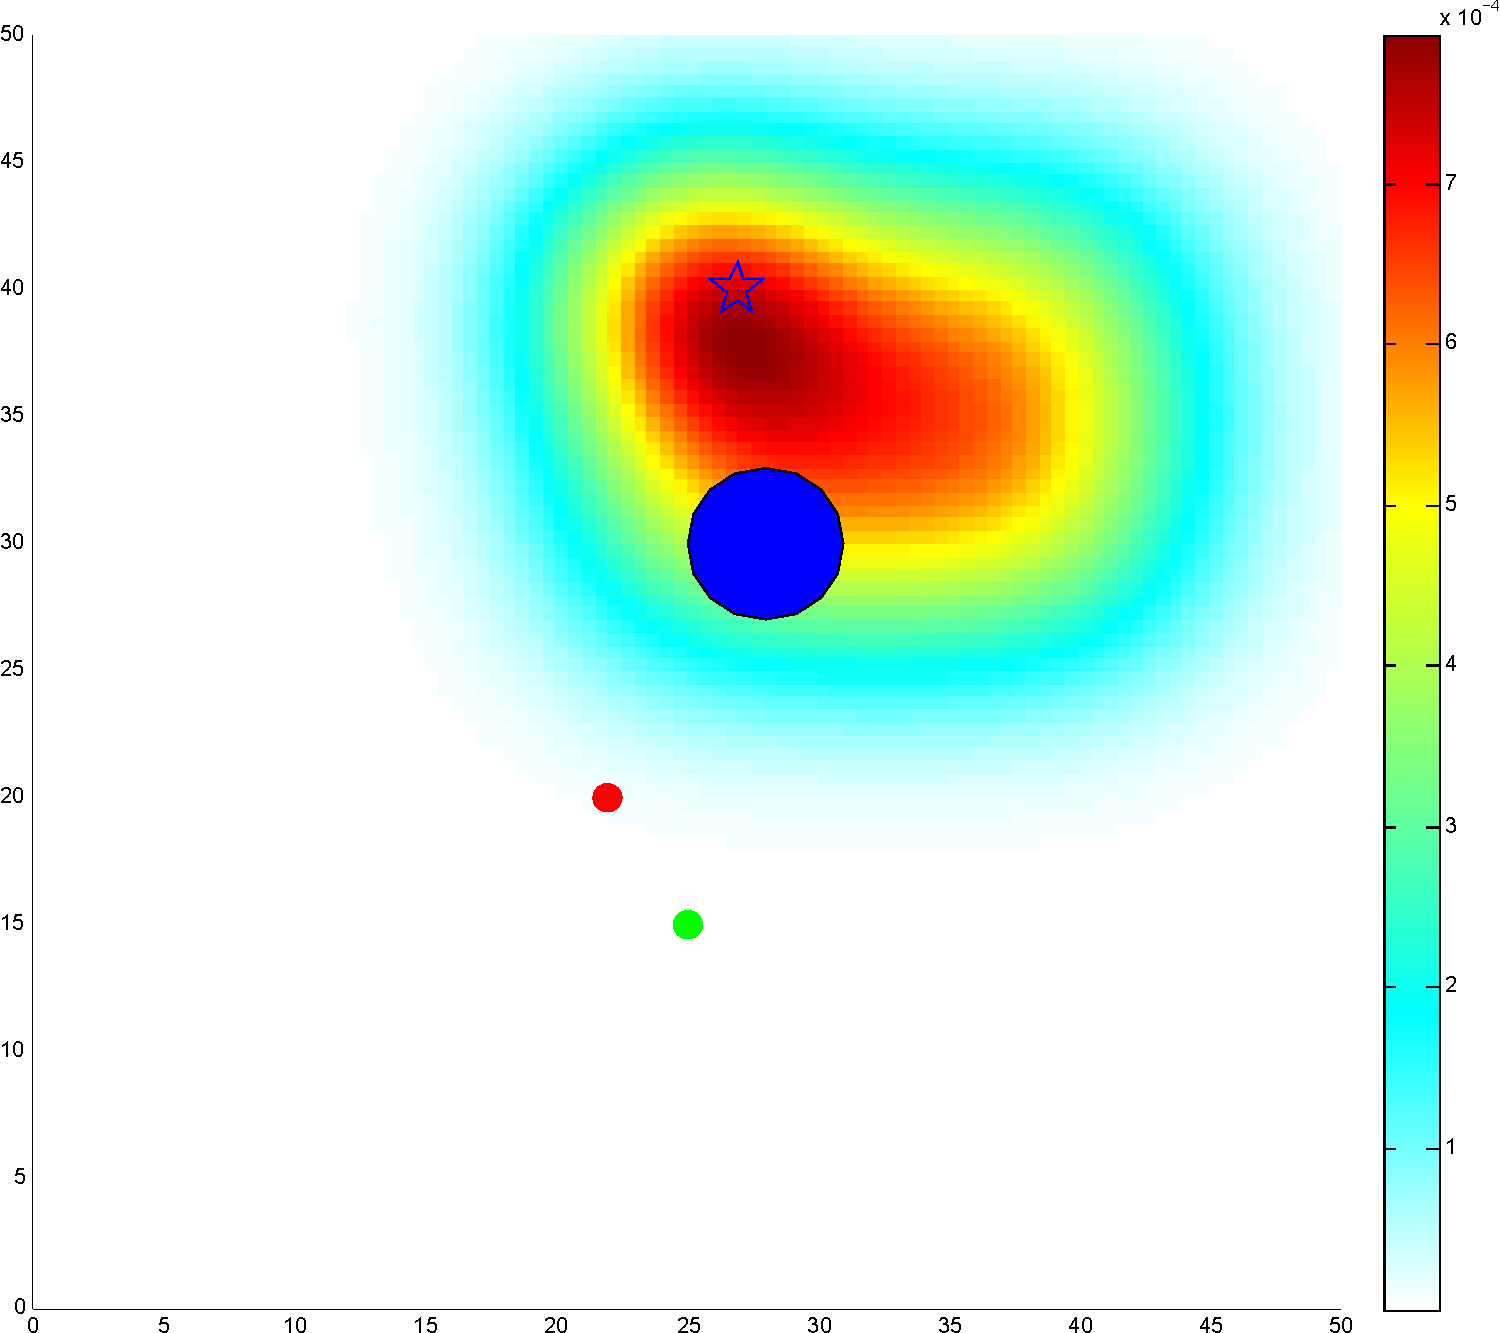
\includegraphics[width=\textwidth]{figures/clt_1_sim1_init_newcm1}
		\caption{}\label{fig:clt_1_sim_init}
	\end{subfigure}
	\begin{subfigure}[b]{0.2\textwidth}
		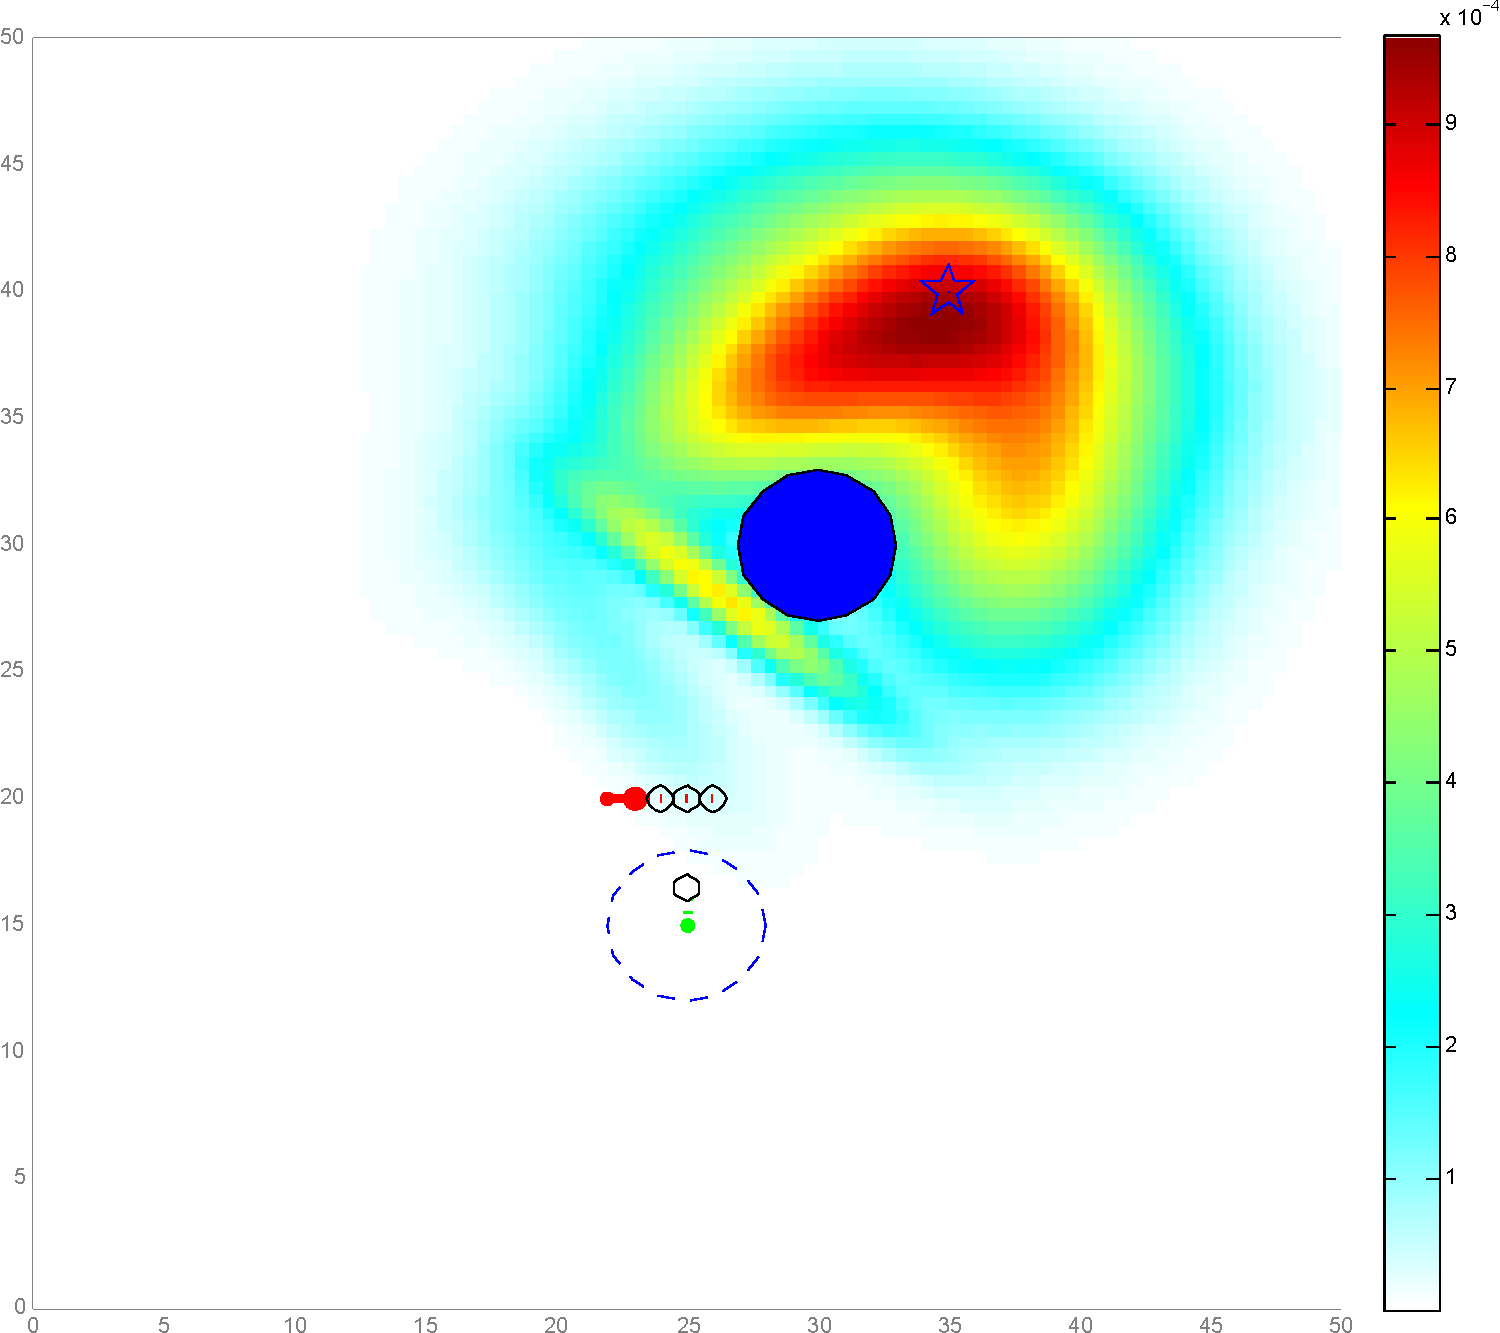
\includegraphics[width=\textwidth]{figures/clt_1_sim1_1ststep_newcm1}
		\caption{}\label{fig:clt_1_sim_1ststep}
	\end{subfigure}
	\begin{subfigure}[b]{0.2\textwidth}
		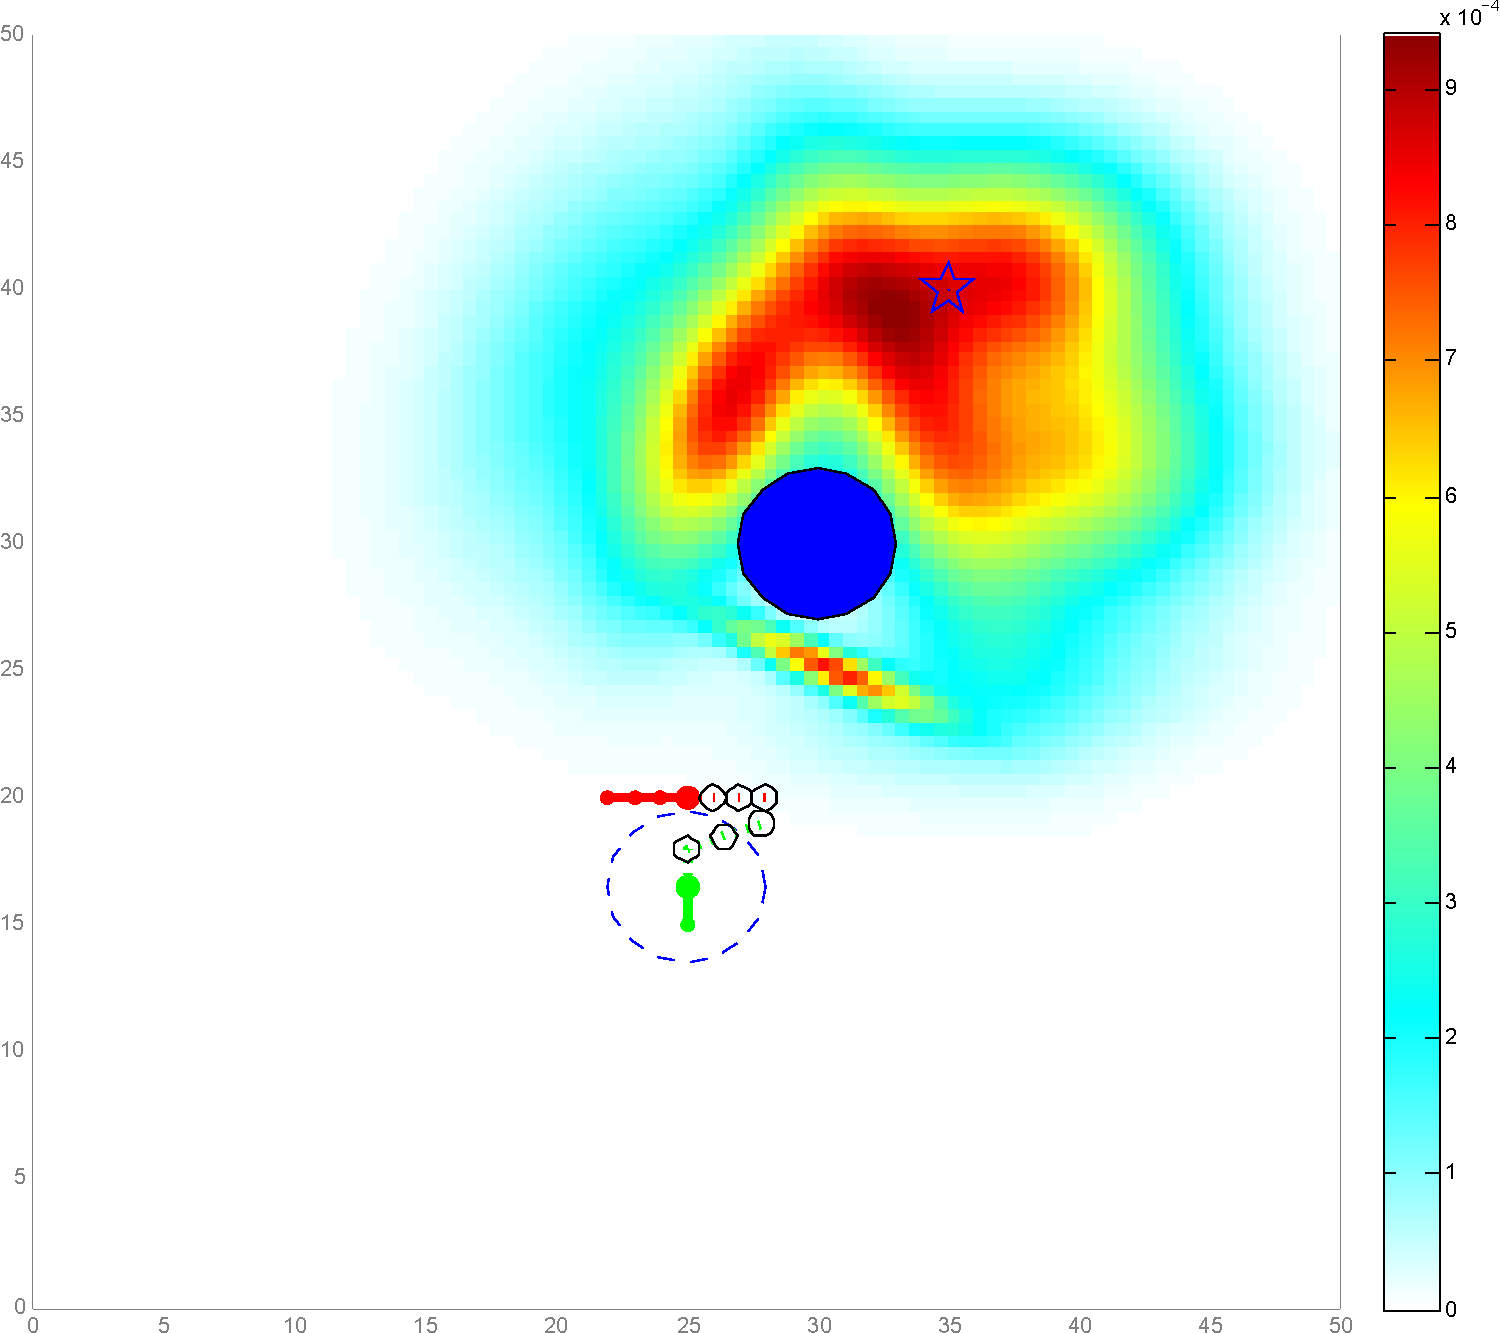
\includegraphics[width=\textwidth]{figures/clt_1_sim1_1_newcm1}
		\caption{}\label{fig:clt_1_sim_avoid_h_1}
	\end{subfigure}
%	\begin{subfigure}[b]{0.2\textwidth}
%		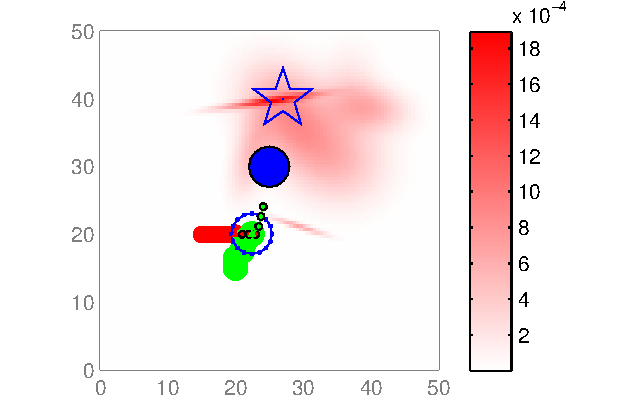
\includegraphics[width=\textwidth]{figures/clt_1_sim2_avoid_h_2}
%		\caption{robot avoids the human}\label{fig:clt_1_sim_avoid_h_2}
%	\end{subfigure}
	\begin{subfigure}[b]{0.2\textwidth}
		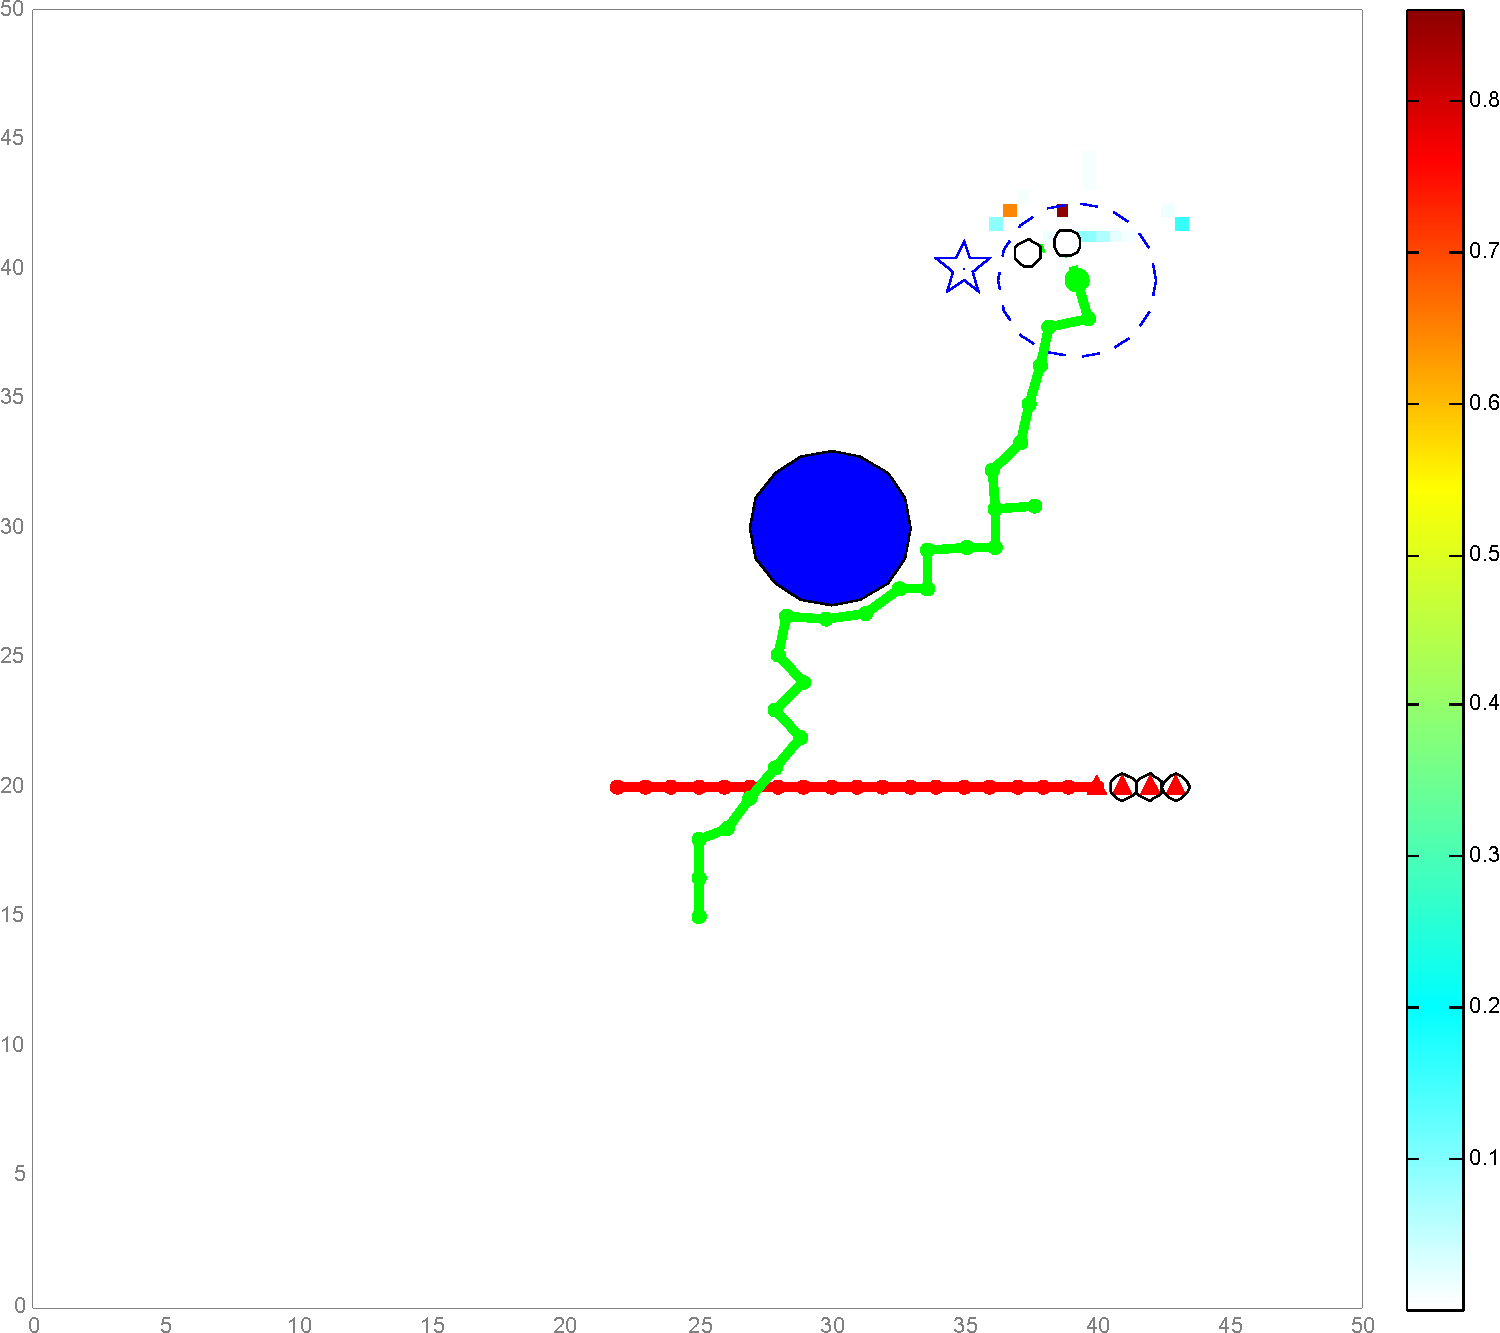
\includegraphics[width=\textwidth]{figures/clt_1_sim1_end_newcm1}
		\caption{}\label{fig:clt_1_sim_end}
	\end{subfigure}
	\caption{\cref{fig:clt_1_sim_init}: the initial layout of the scenario with one high probability density region. \cref{fig:clt_1_sim_1ststep}: the robot starts searching; the red dots with black circles are the predicted trajectory of the moving obstacle and the green ones are the robot's planned trajectory. \cref{fig:clt_1_sim_avoid_h_1}: the robot avoids collision with the human in the prediction horizon. \cref{fig:clt_1_sim_end}: the robot successfully localizes the target.}
\end{figure}

The initial layout of the second scenario is shown in \cref{fig:clt_2_sim_init}, which contains two separate high probability density regions.
The robot starts searching within the lower-left high probability density region, as shown in \cref{fig:clt_2_sim_leave_clt}.
It follows the path that maximizes the probability of detecting the target.
%Recall that the terminal cost function $J_\text{trm} (y^R_{k},u^R_{k:k+H-1})$ \cref{eqn:obj3} drives the robot towards the position with the highest probability density in the probability map.
%However, in this scenario, it is desirable for the robot to search within one high probability density region until the probability densities in that region drop low.
%Therefore, \cref{eqn:obj3} is modified in this case so that it guides the robot towards the high probability density position within the region that the robot is searching.
%This is achieved by clustering the particles based on their positions using the K-means clustering method \cite{hartigan1979algorithm} at the beginning of the search, which results in two separate clusters, one represents the lower-left region and the other represents the upper-right region.
As the robot does not detect the target, the probability density in this region decreases and the robot will leave this region when the probability density drops below a given threshold.
In \cref{fig:clt_2_sim_avoid_ob}, the robot moves towards the top-right high probability region.
It is worth noting that the robot's planned path is along the boundary of the static obstacle, which shows that the collision avoidance is effectively enforced.
%As shown in \cref{fig:clt_2_sim_1ststep}, the robot first searches the lower-left cluster.
%When the probability density in this cluster becomes low, the robot heads for another cluster, as shown in \cref{fig:clt_2_sim_leave_clt}.
%In \cref{fig:clt_2_sim_avoid_h}, the robot has searched along the obstacle with collision with it. 
%Besides, the robot aligns its next three steps with the human's predicted trajectory to avoid hitting the human.
\cref{fig:clt_2_sim_end} shows that the robot has successfully localized the target.

\begin{figure}\label{scenario two}
	\centering
	\begin{subfigure}[b]{0.2\textwidth}
		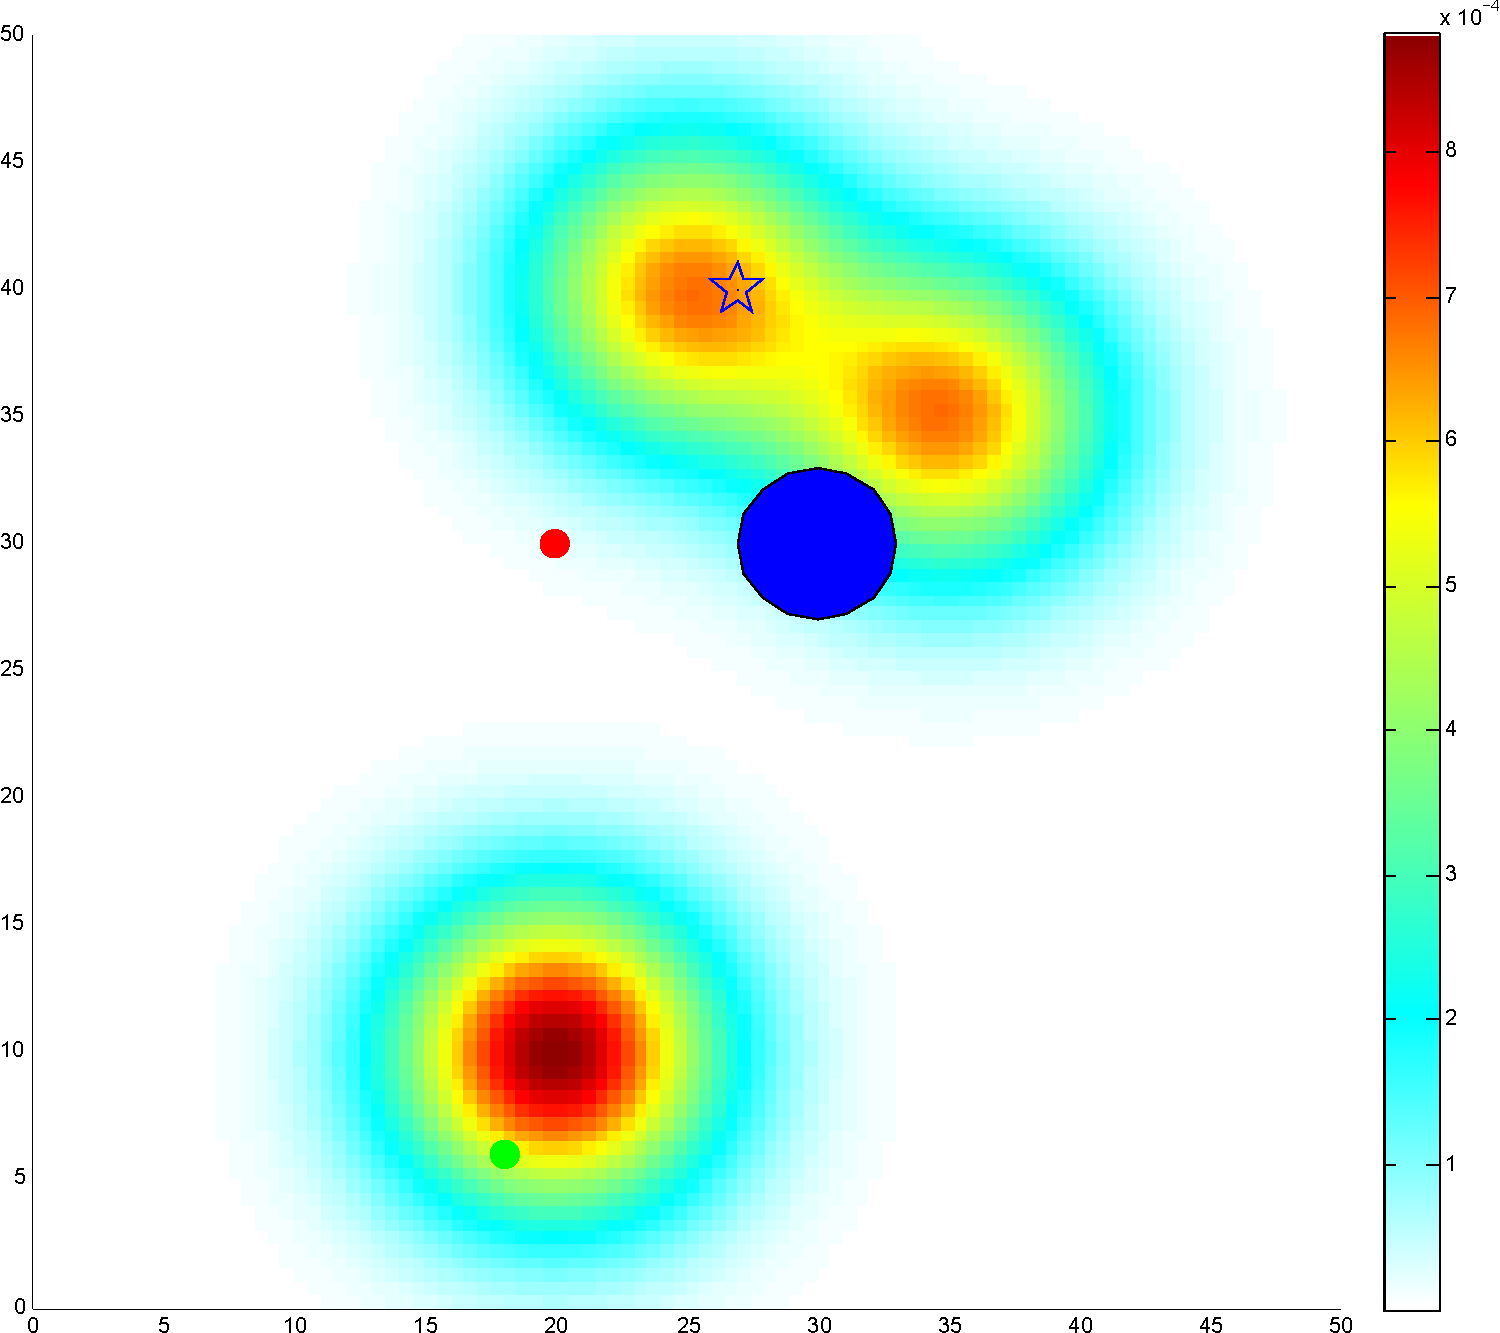
\includegraphics[width=\textwidth]{figures/clt_2_sim3_init_newcm1}
		\caption{}\label{fig:clt_2_sim_init}
	\end{subfigure}
	\begin{subfigure}[b]{0.2\textwidth}
		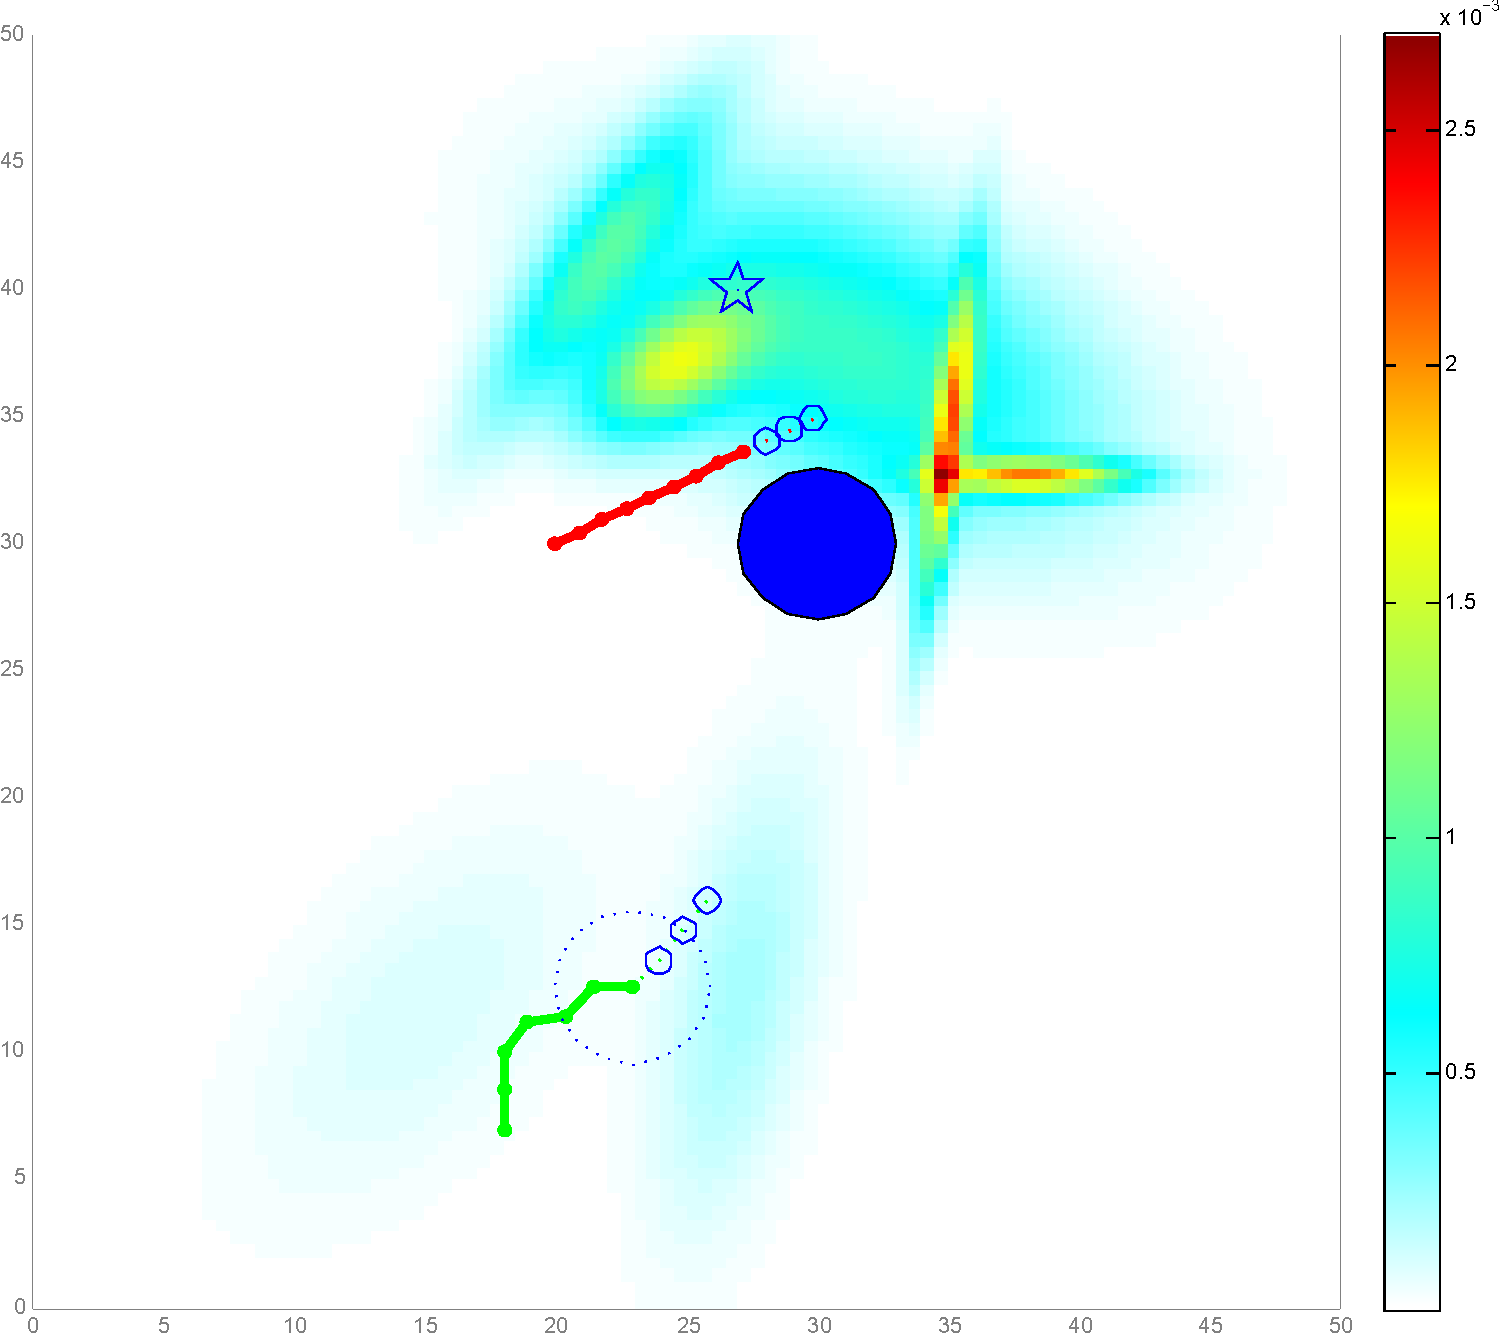
\includegraphics[width=\textwidth]{figures/clt_2_sim3_leave_clt_newcm1}
		\caption{}\label{fig:clt_2_sim_leave_clt}
	\end{subfigure}
	\begin{subfigure}[b]{0.2\textwidth}
		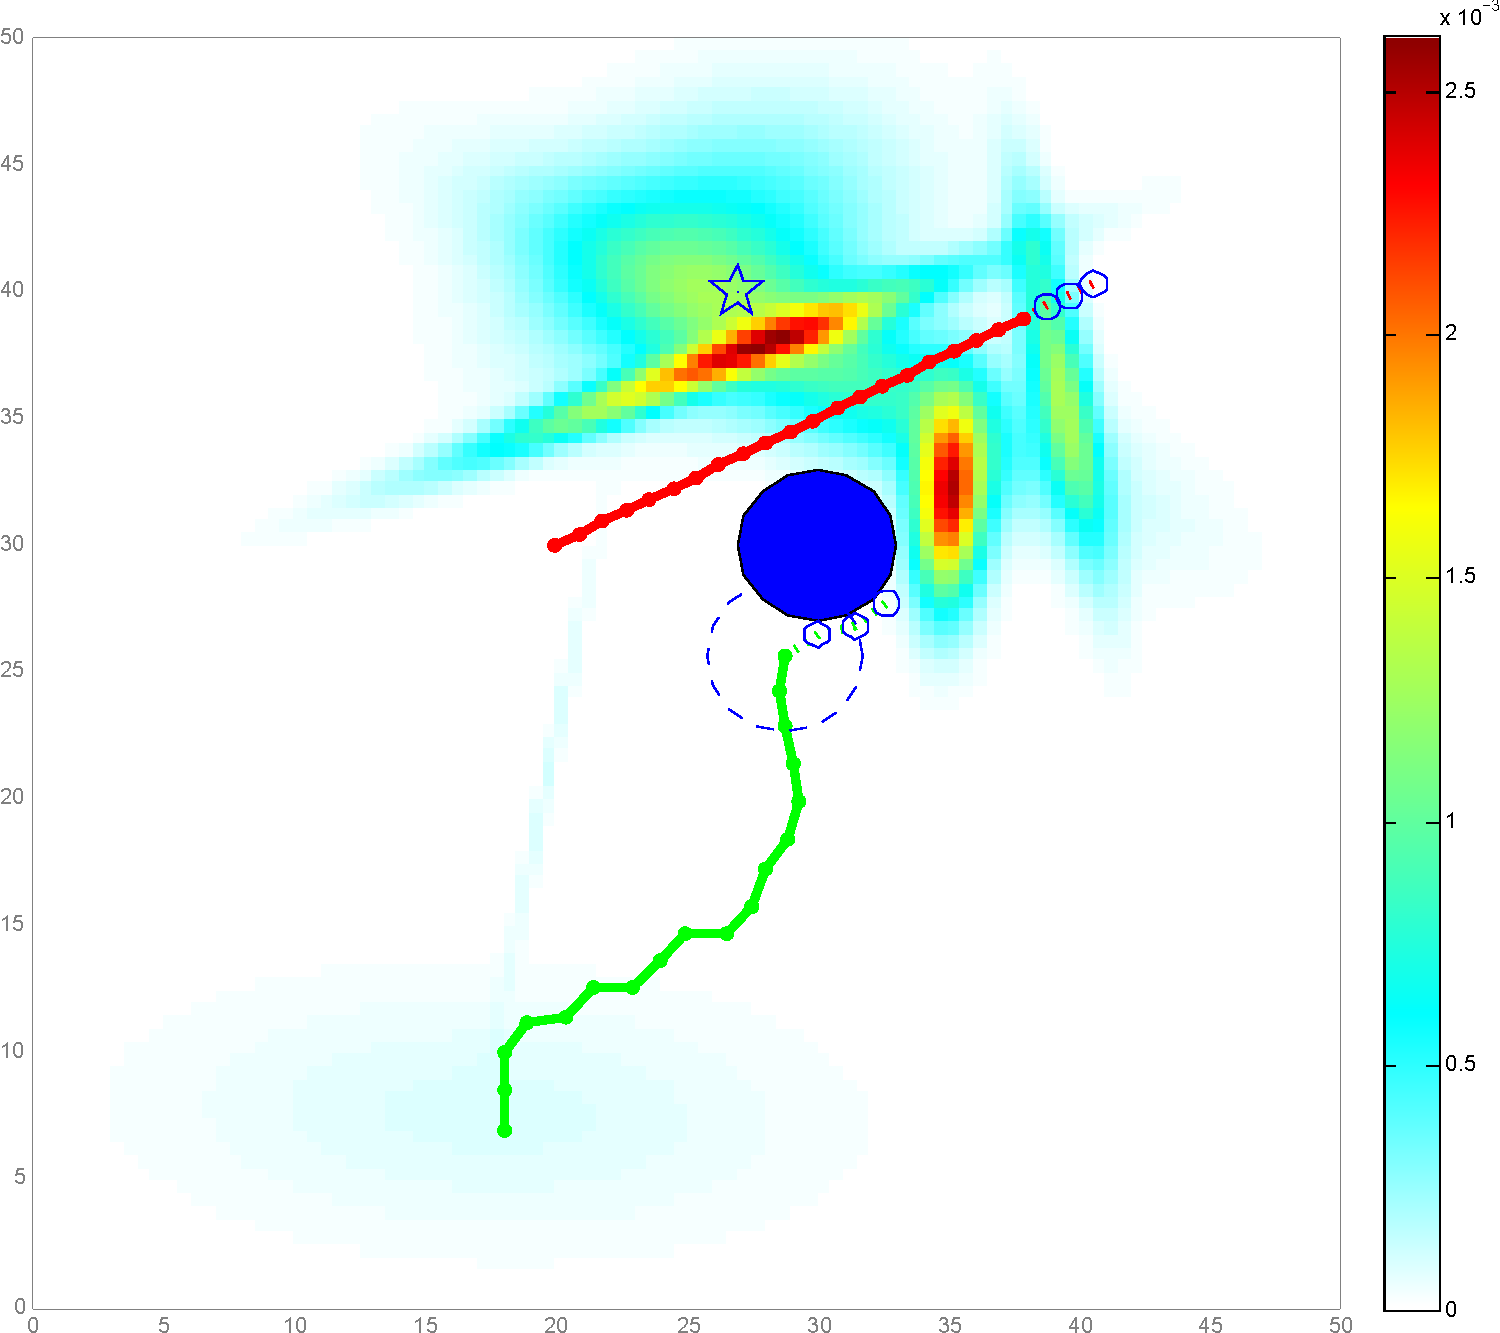
\includegraphics[width=\textwidth]{figures/clt_2_sim3_avoid_ob_1_newcm1}
		\caption{}\label{fig:clt_2_sim_avoid_ob}
	\end{subfigure}
	\begin{subfigure}[b]{0.2\textwidth}
		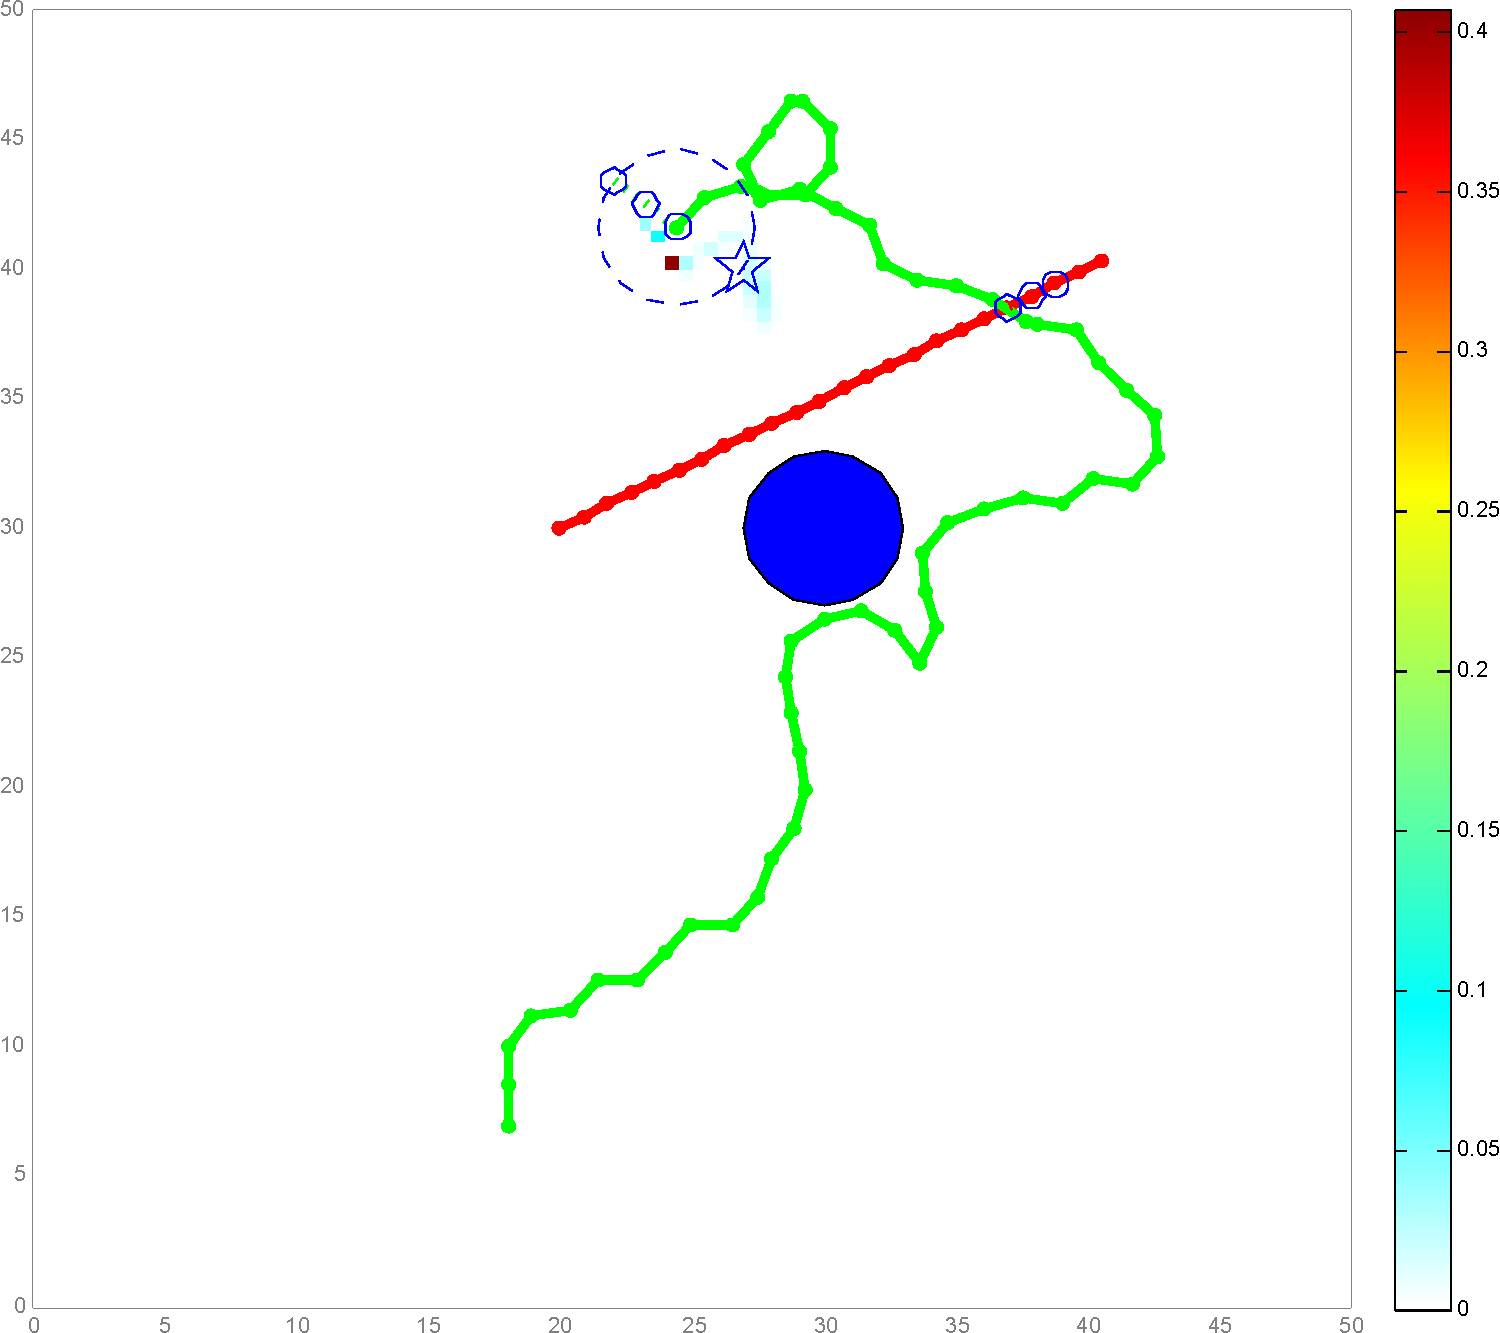
\includegraphics[width=\textwidth]{figures/clt_2_sim3_end_newcm1}
		\caption{}\label{fig:clt_2_sim_end}
	\end{subfigure}
	\caption{\cref{fig:clt_2_sim_init}: the initial layout of the scenario with two high probability density regions. \cref{fig:clt_2_sim_leave_clt}: the robot searches in the lower-left region, following the path that maximizes the probability of detecting the target. \cref{fig:clt_2_sim_avoid_ob}: the robot avoids collision with the static obstacle in the prediction horizon.\cref{fig:clt_2_sim_end}: the robot successfully localizes the target.}
\end{figure}

%The proposed method has been compared using different planning horzions and with the greedy method.
%Using the greedy method, the robot moves along the deepest gradient direction of the probability map.
%\cref{key} compares the average search time, the collision times with obstacles and humans, and the success rate of finding the target within the time limit.

\section*{CONCLUSION}\label{sec:conclusion}
In this work, we proposed an autonomous target search approach using a ground robot to localize a stationary target in a dynamic environment.
%This problem can find applications in scenarios such as the search and rescue. 
%however few works have been done in this area.
A model predictive control (MPC)-based probabilistic search framework is utilized to 
%compute finite-horizon optimal search path based on the probability map to 
maximize the probability of detecting the target while avoiding collision with surrounding obstacles.
The probability map used in the objective function is updated using recursive Bayesian estimation (RBE) and then approximated by a Gaussian Mixture Model (GMM).
%The probabilistic search framework using RBE is utilized to construct and update the probability map.
%RBE is implemented by using the particle filter and the updated probability map is approximated by GMMs.
%%The MPC is utilized to recursively compute a collision-free search path for the robot based on the probability map to maximize the probability of detecting the target.
%The probability map is updated using the particle filtering method and 
An analytical form of the objective function in the prediction horizon is derived for the purpose of allowing a longer prediction horizon and reducing the computation complexity.
%Collision avoidance is enforced by using barrier functions.
Simulations have shown the effectiveness of the proposed method for a robot to autonomously search the target while avoiding collision with both static and moving obstacles.

Future work may include several extensions to the proposed method.
%First, current objective function is non-convex and nonlinear, which incurs high computation complexity.
%and no guarantee of globally optimal solution.
%Speedup may be achieved by implementing the convex relaxation of the objective function and applying the branch-and-bound method.
%Second, the feasibility and stability of the MPC needs investigation.
%First, in this paper, the effectiveness of the method is demonstrated through simulations.
For MPC-based search framework, A thorough study of the feasibility and stability is still necessary for practical applications.
%In addition, a simple motion model is utilized for predicting the trajectory of moving obstacles.
In addition, many obstacles may have more complex motion patterns. A more realistic motion prediction model is also needed.

\section*{ACKNOWLEDGMENT}
This work is part of the Embedded Humans: Provably Correct Decision Making for Networks of Humans and Unmanned Systems project, a MURI project funded by the Office of Naval Research.
%The authors would like to thank Professor Tom Griffiths from the Department of Psychology at the University of California, Berkeley for his suggestion on the goal inference method. 
%The authors also would like to thank Romain Jacob and Jared Garvey for their helpful discussions.

\appendix
\section*{APPENDIX A}\label{append_a}

\subsection*{Exponential Family of Distributions}\label{app:exp_family}
%In this section, we provide the necessary explanation of the Exponential Family of Distributions as we will use them to describe the analytical form of the objective function in \cref{sec:explicit_form}.
In this section, we present the procedure to reformulating a multi-variate Gaussian distribution into the form of the Exponential Family.
The Exponential Family of Distributions is defined as
\begin{equation}\label{eqn:exp_family_app}
g(x;\theta)=h(x)e^{\eta(\theta)^TT(x)-A(\theta)},
\end{equation}
where $x$ and $\theta$ represent variables and parameters respectively.
%A multi-variate Gaussian distribution belongs to the Exponential Family.
%and can be written in the form of \cref{eqn:exp_family}.
A $d$-dimensional Gaussian distribution with the known mean $\mu$ and covariance $\Sigma$ is defined as
\begin{equation*}
q(x;\mu,\Sigma)=(2\pi)^{-\frac{d}{2}}|\Sigma|^{-\frac{1}{2}}e^{-\frac{1}{2}(x-\mu)^T\Sigma^{-1}(x-\mu)}.
\end{equation*}

The equation $q(x;\mu,\Sigma)$ can be written in the form of \cref{eqn:exp_family_app} with the following parameters:
\begin{subequations}\label{eqn:N2exp_para_app}
	\begin{align}
	\theta&=\left[\mu,\Sigma\right],\\
	T(x)&=\left[ x,-xx^T\right]^T,\\
	\eta(\theta)&=\left[\Sigma^{-1}\mu,\frac{1}{2}\Sigma^{-1}\right]^T, \label{symb:eta_theta}\\
	h(x)&=1,\\
	A(\theta)&=\frac{1}{2}\mu^T\Sigma^{-1}\mu+\frac{1}{2}|\Sigma|+\frac{d}{2}ln(2\pi).\label{symb:A_theta}
	\end{align}
\end{subequations}

Define 
\begin{subequations}
	\begin{align}
	\Lambda&=\Sigma^{-1}\mu, \label{symb:Lambda_app}\\
	\Psi&=\frac{1}{2}\Sigma^{-1}. \label{symb:Psi_app}
	\end{align}
\end{subequations}

Let $\Phi = \left[\Lambda,\Psi\right]$.
Notice that \cref{symb:Lambda_app} and \cref{symb:Psi_app} correspond to $\eta(\theta)$ in \cref{symb:eta_theta}.
Then $q(x;\mu,\Sigma)$ can be reformulated using $\Phi$ as the parameter:
\begin{equation*}%\label{eqn:gau_phi_app}
q(x;\Phi)=e^{\Phi^TT(x)-A(\Phi)},
\end{equation*}
where
\begin{equation*}
A(\Phi)=\frac{1}{4}\Lambda^T\Psi^{-1}\Lambda+\frac{d}{2}ln(2\pi)-\frac{1}{2}|2\Psi|\label{symb:A_Phi_app}.
\end{equation*}
%Therefore the parameter of a Gaussian distribution can be represented in terms of $\Phi$ instead of $\theta=\left[\mu,\Sigma\right]$.
%We will use $\Phi$ as the parameter for Gaussian distributions in the rest of the paper.

\section*{APPENDIX B}\label{append_b}
\subsection*{Deriving the Analytical form of the Objective Function}
%\subsection*{Analytical Form of the Objective Function}
%In the appendix, a well-known property of Gaussian distributions is presented using the form of the Exponential Family.
%Then the analytical form of the objective function is derived.
It is known that the product of two Gaussian probability density functions (PDFs) is a Gaussian function (not a Gaussian PDF).
To be specific, let $f(x)$ and $g(x)$ be two Gaussian PDFs in the form of \cref{eqn:gau_phi_app}:
\begin{subequations}
	\begin{align*}
	f(x)&=e^{\Phi_1^TT(x)-A(\Phi_1)},\\
	g(x)&=e^{\Phi_2^TT(x)-A(\Phi_2)}.
	\end{align*}
\end{subequations}
%Note the $h(x)$ in \cref{eqn:gau_phi_app} is omitted as its value is 1 for a Gaussian PDF.

Their product is
\begin{align}
r(x)&=f(x)g(x)\notag\\&=e^{(\Phi_1+\Phi_2)^TT(x)-A(\Phi_1)-A(\Phi_2)}\notag\\
&=e^{A(\Phi_1+\Phi_2)-A(\Phi_1)-A(\Phi_2)}e^{(\Phi_1+\Phi_2)^TT(x)-A(\Phi_1+\Phi_2)}\notag\\
&=se^{(\Phi_1+\Phi_2)^TT(x)-A(\Phi_1+\Phi_2)}.\notag
\end{align}
where $s=e^{A(\Phi_1+\Phi_2)-A(\Phi_1)-A(\Phi_2)}$ is a constant.
Therefore $r(x)$ is a Gaussian function with the parameter $\Phi_1+\Phi_2$.
This closure property is applied to the non-detection function \cref{eqn:sub}.
%\cref{eqn:obj_int}.
%Recall that the probability map is approximated as a GMM \cref{eqn:gmm_prob_map_exp_fam} and the sensor model is a Gaussian function \cref{eqn:sensor_model}.
%\begin{align}
%J_{pnd}(y^R_k,u^R_{k:k+H-1})&=\int_S P(x^t|y^R_{k})\prod\limits_{i=1}^H P(z_{k+i}=\mathbf{0}|x^t,y^R_{k+i})\mathrm{d}x^t\\
%&=\int_S \sum\limits_{j=1}^{n}v_j e^{\Phi_{j,k}^TT(x^t)-A(\Phi_{j,k})}\notag\\ &\prod\limits_{i=1}^{H}\left[ 1-ce^{{\Phi^R_{k+i}}^TT(x^t)-A(\Phi^R_{k+i})}\right] \mathrm{d}x^t,
%\end{align}
%where $\Phi_{j,k}=\left[ \Sigma^{-1}_{j,k}\mu_{j,k},\frac{1}{2} \Sigma^{-1}_{j,k}\right] $ is the parameter for the $j^\text{th}$ Gaussian distribution in \cref{eqn:gmm_prob_map}, using the notation of the Exponential Family.
For the purpose of simplicity, we derive the case of $H=2$.
\begin{subequations}
	\begin{align}
	J(y^R_k,u^R_{k:k+1})&=\int_S \sum\limits_{j=1}^{n}v_j e^{\Phi_{j,k}^TT(x^t)-A(\Phi_{j,k})}\notag\\ &\prod\limits_{i=1}^{2}\left[ 1-ce^{{\Phi^R_{k+i}}^TT(x^t)-A(\Phi^R_{k+i})}\right] \mathrm{d}x^t,\\
	&=\int_S \sum\limits_{j=1}^{n}v_j e^{\Phi_{j,k}^TT(x^t)-A(\Phi_{j,k})}\notag\\
	&\big[ 1-ce^{{\Phi^R_{k+1}}^TT(x^t)-A(\Phi^R_{k+1})}-ce^{{\Phi^R_{k+2}}^TT(x^t)-A(\Phi^R_{k+2})}\notag\\&+c^2e^{(\Phi^R_{k+1}+\Phi^R_{k+2})^TT(x^t)-A(\Phi^R_{k+1})-A(\Phi^R_{k+2})}\big] \mathrm{d}x^t\notag\\
	&=\sum\limits_{j=1}^{n}v_j \int_S e^{\Phi_{j,k}^TT(x^t)-A(\Phi_{j,k})}\notag\\
	&\big[ 1-ce^{{\Phi^R_{k+1}}^TT(x^t)-A(\Phi^R_{k+1})}-ce^{{\Phi^R_{k+2}}^TT(x^t)-A(\Phi^R_{k+2})}\notag\\&+c^2e^{(\Phi^R_{k+1}+\Phi^R_{k+2})^TT(x^t)-A(\Phi^R_{k+1})-A(\Phi^R_{k+2})}\big] \mathrm{d}x^t\label{eqn:obj_2step_app}.
	\end{align}
\end{subequations}


Consider the following integral \cref{eqn:one_part_integ_app} that appears as one part of the integral term associated with $v_j$ in \cref{eqn:obj_2step_app}.
It can be simplified as follows:
\begin{align}
&\int_S e^{{\Phi_{j,k}}^TT(x^t)-A(\Phi_{j,k})}\,e^{{\Phi^R_{k+1}}^TT(x^t)-A(\Phi^R_{k+1})} \mathrm{d}x^t\label{eqn:one_part_integ_app}\\
&=\int_S e^{{(\Phi_{j,k}+\Phi^R_{k+1})}^TT(x^t)-A(\Phi_{j,k})-A(\Phi^R_{k+1})} \mathrm{d}x^t,\\
&=e^{A(\Phi_{j,k}+\Phi^R_{k+1})-A(\Phi_{j,k})-A(\Phi^R_{k+1})}\int_S e^{(\Phi_{j,k}+\Phi^R_{k+1})^TT(x^t)-A(\Phi_{j,k}+\Phi^R_{k+1})} \mathrm{d}x^t\label{eqn:integ_out_app},\\
&=e^{A(\Phi_{j,k}+\Phi^R_{k+1})-A(\Phi_{j,k})-A(\Phi^R_{k+1})}. \label{eqn:no_integ_app}
\end{align}

Equation \cref{eqn:no_integ_app} is obtained from \cref{eqn:integ_out_app} since the exponential term to be integrated is a Gaussian probability density function, the integral of which equals 1.

Define
\begin{subequations}
	\begin{align*}
	\alpha_{j,i_1}&=A(\Phi_{j,k}+\Phi^R_{k+1})-A(\Phi_{j,k})-A(\Phi^R_{k+1}),\\
	\alpha_{j,i_2}&=A(\Phi_{j,k}+\Phi^R_{k+2})-A(\Phi_{j,k})-A(\Phi^R_{k+2}),\\
	\alpha_{j,i_1,i_2}&=A(\Phi_{j,k}+\Phi^R_{k+1}+\Phi^R_{k+2})-A(\Phi_{j,k})-A(\Phi^R_{k+1})-A(\Phi^R_{k+2}).
	\end{align*}
\end{subequations}

Then using similar method for deriving \cref{eqn:no_integ_app}, equation \cref{eqn:obj_2step_app} can be simplified as
\begin{equation*}
J(u_{k:k+1})=1+\sum\limits_{j=1}^{n}[-cv_je^{\alpha_{j,i_1}}-cv_je^{\alpha_{j,i_2}}+c^2v_je^{\alpha_{j,i_1,i_2}}].
\end{equation*}

The general formula of the non-detection function with horizon $H$ is shown in \cref{eqn:exp_obj_H}.
\bibliographystyle{asmems4}
\bibliography{references}
\end{document}
